% !TeX program = pdflatex
% !BIB program = biber
% !TeX encoding = UTF-8 Unicode

\documentclass[12pt,a4paper]{article}

% ============================================================
% Configuración general
% ============================================================

\usepackage[T1]{fontenc}
\usepackage[utf8]{inputenc}
\usepackage[spanish,es-nodecimaldot]{babel}

% Tipografía académica: serif para cuerpo y sans serif para jerarquía
\usepackage{newtxtext,newtxmath}
\usepackage[scaled=0.92]{helvet}
\usepackage{microtype}

\usepackage[
    top=2.55cm,
    bottom=2.55cm,
    left=3.00cm,
    right=2.55cm,
    headheight=15pt,
    headsep=0.75cm,
    footskip=1.20cm
]{geometry}

\usepackage{setspace}
\setstretch{1.15}

\setlength{\parindent}{1.15em}
\setlength{\parskip}{0.18em}
\raggedbottom

% ============================================================
% Colores: paleta original de inspiración académica británica
% ============================================================

\usepackage{xcolor}

\definecolor{AcademicNavy}{HTML}{17324D}
\definecolor{AcademicTeal}{HTML}{6F9390}
\definecolor{AcademicSlate}{HTML}{4A5561}
\definecolor{AcademicMist}{HTML}{EEF2F3}
\definecolor{AcademicRule}{HTML}{C9D1D6}

% ============================================================
% Matemáticas, tablas y figuras
% ============================================================

\usepackage{amsmath}
\usepackage{amssymb}
\usepackage{mathtools}

\usepackage{booktabs}
\usepackage{tabularx}
\usepackage{longtable}
\usepackage{array}
\usepackage{multirow}
\usepackage{threeparttable}

\usepackage{graphicx}
\usepackage{float}
\usepackage{subcaption}
\usepackage[section]{placeins}

\graphicspath{
    {../resultados/figuras/}
}

\usepackage{siunitx}
\sisetup{
    output-decimal-marker = {,},
    group-separator = {.},
    group-minimum-digits = 4
}

% ============================================================
% Títulos, listas, pies y navegación
% ============================================================

\usepackage{titlesec}
\usepackage{enumitem}
\usepackage{caption}
\usepackage{fancyhdr}

\titleformat{\section}
    {\Large\sffamily\bfseries\color{AcademicNavy}}
    {\thesection}
    {0.75em}
    {}

\titleformat{\subsection}
    {\large\sffamily\bfseries\color{AcademicSlate}}
    {\thesubsection}
    {0.70em}
    {}

\titleformat{\subsubsection}
    {\normalsize\sffamily\bfseries\color{AcademicSlate}}
    {\thesubsubsection}
    {0.65em}
    {}

\titlespacing*{\section}{0pt}{2.2ex plus 0.7ex minus 0.3ex}{1.2ex}
\titlespacing*{\subsection}{0pt}{1.8ex plus 0.5ex minus 0.2ex}{0.8ex}

\setlist[itemize]{
    leftmargin=1.6em,
    itemsep=0.25em,
    topsep=0.35em
}

\setlist[enumerate]{
    leftmargin=1.8em,
    itemsep=0.25em,
    topsep=0.35em
}

\captionsetup{
    font=small,
    labelfont={bf,sf,color=AcademicNavy},
    textfont=small,
    justification=justified,
    singlelinecheck=false,
    skip=7pt
}

\pagestyle{fancy}
\fancyhf{}
\fancyhead[L]{\sffamily\small MCC002 \textperiodcentered\ Grupo 5}
\fancyhead[R]{\sffamily\small\nouppercase{\leftmark}}
\fancyfoot[C]{\sffamily\small\thepage}

\renewcommand{\headrulewidth}{0.35pt}
\renewcommand{\footrulewidth}{0pt}

% ============================================================
% Bibliografía e hipervínculos
% ============================================================

\usepackage{csquotes}
\usepackage[
    backend=biber,
    style=apa,
    sorting=nyt,
    maxcitenames=2,
    maxbibnames=99
]{biblatex}

\usepackage[
    colorlinks=true,
    linkcolor=AcademicNavy,
    citecolor=AcademicNavy,
    urlcolor=AcademicTeal,
    pdfborder={0 0 0}
]{hyperref}

\hypersetup{
    pdftitle={Informe final MCC002 - Grupo 5},
    pdfauthor={Armando Castro Chaupis, Henry Sánchez Alvarado y Alex Segura Núñez},
    pdfsubject={Riesgo crediticio y predicción cuantitativa},
    pdfkeywords={riesgo crediticio, regresión logística, inferencia, Bayes, German Credit Data}
}

% ============================================================
% Entornos propios
% ============================================================

\newenvironment{hallazgo}
{
    \begin{quote}
    \color{AcademicNavy}
    \sffamily
    \textbf{Hallazgo principal.}\;
}
{
    \end{quote}
}

\newcommand{\variable}[1]{\texttt{#1}}
\newcommand{\pvalor}{\ensuremath{p\text{-valor}}}
\newcommand{\AUC}{\ensuremath{\mathrm{AUC}}}
\newcommand{\OR}{\ensuremath{\mathrm{OR}}}

% Control tipográfico
\widowpenalty=10000
\clubpenalty=10000
\displaywidowpenalty=10000
\emergencystretch=2em

% ============================================================
% Metadatos editables del informe
% ============================================================

\newcommand{\Universidad}{Universidad Nacional de Ingeniería}
\newcommand{\Facultad}{Facultad de Ciencias}
\newcommand{\Programa}{Maestría en Ciencia de la Computación}
%\newcommand{\Mencion}{Mención en Computación Científica}

\newcommand{\Curso}{MCC002 --- Probabilidad y Estadística Computacional}
\newcommand{\Docente}{Dra. Rocío Milagros Zorrilla Coz}
\newcommand{\Periodo}{Periodo Académico 2026-1}
\newcommand{\Grupo}{Grupo 5}

% Título provisional; se puede ajustar antes de cerrar la Sección 1.
\newcommand{\TituloInforme}{
    Riesgo y Predicción Cuantitativa
}

\newcommand{\SubtituloInforme}{
    Análisis Predictivo del Statlog German Credit Data
}

\newcommand{\IntegranteUno}{Armando Castro Chaupis}
\newcommand{\IntegranteDos}{Henry Sánchez Alvarado}
\newcommand{\IntegranteTres}{Alex Segura Núñez}

\newcommand{\CiudadFecha}{Lima, Perú --- 2026}


\addbibresource{referencias.bib}

\begin{document}

\begin{titlepage}
    \thispagestyle{empty}

    \color{AcademicNavy}
    \rule{\textwidth}{1.2pt}

    \vspace{0.65cm}

    {\sffamily\bfseries\large \Universidad\par}
    \vspace{0.15cm}
    {\sffamily\normalsize \Facultad\par}
    {\sffamily\normalsize \Programa\par}
    {\sffamily\normalsize \Mencion\par}

    \vfill

    {\sffamily\small\bfseries\MakeUppercase{\Curso}\par}

    \vspace{1.0cm}

    {\fontsize{24}{29}\selectfont\bfseries
        \TituloInforme
        \par
    }

    \vspace{0.55cm}

    {\large\color{AcademicSlate}
        \SubtituloInforme
        \par
    }

    \vspace{0.8cm}

    {\color{AcademicTeal}\rule{0.28\textwidth}{2.1pt}\par}

    \vfill

    \begin{tabularx}{\textwidth}{@{}>{\sffamily\bfseries}l X@{}}
        Trabajo & Trabajo Práctico Final Integrador \\
        Equipo & \Grupo \\
        Integrantes &
            \IntegranteUno \newline
            \IntegranteDos \newline
            \IntegranteTres \\
        Docente & \Docente \\
        Periodo & \Periodo \\
    \end{tabularx}

    \vfill

    {\sffamily\small\color{AcademicSlate}\CiudadFecha\par}

    \vspace{0.35cm}
    \color{AcademicNavy}
    \rule{\textwidth}{0.55pt}
\end{titlepage}


\pagenumbering{roman}
\section*{Resumen}
\addcontentsline{toc}{section}{Resumen}

% Texto provisional. Se cerrará cuando todas las secciones estén terminadas.
Este informe estudia los factores asociados con la clasificación de un
solicitante como mal riesgo crediticio mediante el conjunto
\textit{Statlog German Credit Data}. El análisis integra estadística
descriptiva, inferencia frecuentista, regresión lineal y logística,
evaluación predictiva bajo costos asimétricos e inferencia bayesiana. El
objetivo es producir conclusiones cuantitativas defendibles sobre la tasa
de mal crédito, las diferencias entre perfiles de solicitantes y el efecto
del umbral de decisión sobre la clasificación. Las estimaciones y
visualizaciones se generan de forma reproducible desde el notebook del
proyecto.

\medskip

\noindent
\textbf{Palabras clave:}
riesgo crediticio; regresión logística; costos asimétricos; inferencia
frecuentista; inferencia bayesiana; German Credit Data.


\tableofcontents
\clearpage

\listoffigures
\addcontentsline{toc}{section}{Índice de figuras}
\clearpage

\listoftables
\addcontentsline{toc}{section}{Índice de tablas}
\clearpage

\pagenumbering{arabic}
\setcounter{page}{1}

\section{Introducción y pregunta de investigación}
\label{sec:introduccion}

% Contenido previsto:
% - Contexto del riesgo de crédito.
% - Problema de decisión y costo de errores.
% - Pregunta central del Grupo 5.
% - Cinco preguntas secundarias.
% - Objetivo general y objetivos específicos.
% - Alcance: asociación y predicción, no causalidad.

\section{Descripción y citación del dataset}
\label{sec:dataset}

% Contenido previsto:
% - Statlog German Credit Data.
% - Fuente, autor, año, DOI y licencia.
% - Número de observaciones y variables.
% - Formato original german.data.
% - Matriz de costos 5:1.
% - Pertinencia y límites de representatividad.

\section{Diccionario de variables}
\label{sec:diccionario}

% Contenido previsto:
% - Tabla completa de las 20 variables predictoras y la respuesta.
% - Tipo, unidad, codificación original, nombre analítico y transformación.
% - Recodificación explícita: 1 = buen riesgo; 2 = mal riesgo.
% - Variable de modelado: 0 = buen riesgo; 1 = mal riesgo.

\section{Limpieza y preprocesamiento}
\label{sec:preprocesamiento}

El preprocesamiento tuvo como propósito construir una base analítica
consistente sin alterar innecesariamente la información original. El
procedimiento se diseñó para ser reproducible, de modo que el notebook
pueda ejecutarse desde el inicio tanto si el dataset ya se encuentra en
el repositorio como si debe descargarse desde la fuente oficial.

A diferencia de otros problemas aplicados, el conjunto de datos no
requirió imputación, eliminación de registros ni corrección manual de
categorías. El trabajo se concentró en verificar la integridad de la
fuente, documentar la codificación de la respuesta, conservar la
naturaleza estadística de los predictores y construir las variables
derivadas necesarias para el análisis.

\subsection{Configuración reproducible}

Al inicio del notebook se fija una semilla global:

\[
\texttt{SEED}=2026.
\]

La semilla se utiliza en los procedimientos que dependen de generación
seudoaleatoria, entre ellos el remuestreo bootstrap, la separación de
datos, la validación cruzada y el sampler Metropolis--Hastings. Su uso
permite reproducir las principales estimaciones obtenidas durante el
análisis.

El entorno utilizado corresponde a Python 3.12.10. Las versiones
registradas durante la ejecución se presentan en la
Tabla~\ref{tab:entorno-computacional}.

\begin{table}[H]
    \centering
    \caption{Entorno computacional registrado por el notebook.}
    \label{tab:entorno-computacional}

    \begin{tabular}{lc}
        \toprule
        Componente & Versión \\
        \midrule
        Python & 3.12.10 \\
        NumPy & 2.4.6 \\
        pandas & 3.0.3 \\
        SciPy & 1.17.1 \\
        statsmodels & 0.14.6 \\
        scikit-learn & 1.9.0 \\
        seaborn & 0.13.2 \\
        \bottomrule
    \end{tabular}
\end{table}

Las dependencias del proyecto se registran adicionalmente en el archivo
\texttt{requirements.txt}. Esta separación entre código, datos,
resultados y dependencias reduce la dependencia del entorno local desde
el cual se ejecuta el análisis.

\subsection{Localización y carga del archivo}

El notebook no utiliza una ruta absoluta fija. En su lugar, busca la raíz
del repositorio recorriendo el directorio actual y sus directorios
superiores hasta encontrar la carpeta \texttt{.git} o el archivo
\texttt{README.md}. A partir de esa ubicación se define la ruta:

\begin{center}
    \texttt{data/german.data}
\end{center}

Si el archivo no se encuentra localmente, el procedimiento descarga el
paquete comprimido desde UCI, verifica que contenga
\texttt{german.data}, lo extrae y lo almacena en la carpeta
\texttt{data}. De esta manera, el notebook puede ejecutarse sin depender
de una copia manual ubicada fuera del proyecto.

El archivo original está separado por espacios y no contiene nombres de
columnas. Durante la lectura se asignan los veintiún nombres definidos
en el diccionario de variables: veinte predictores y la clase original.

Después de la carga se comprueba que la matriz tenga exactamente:

\[
1000\ \text{observaciones}
\quad \times \quad
21\ \text{columnas}.
\]

La ejecución se detiene mediante una excepción si las dimensiones no
coinciden con la documentación o si la variable
\variable{clase} contiene valores diferentes de \(1\) y \(2\).

\subsection{Conservación de los códigos originales}

Las variables categóricas se mantienen con sus códigos originales, por
ejemplo \texttt{A11}, \texttt{A34} o \texttt{A65}. Esta decisión conserva
la trazabilidad con la documentación de UCI y evita modificar la
información antes de definir el uso de cada predictor.

Para facilitar la lectura de tablas y visualizaciones se generan
etiquetas en español para cuatro variables especialmente relevantes:

\begin{itemize}
    \item propósito del crédito;
    \item estado de la cuenta corriente;
    \item nivel de ahorros;
    \item historial crediticio.
\end{itemize}

Las nuevas columnas utilizan el sufijo \texttt{\_lbl}. Por ejemplo,
\variable{proposito_lbl} contiene descripciones como ``Auto nuevo'',
``Educación'' o ``Negocio'', mientras que
\variable{proposito} conserva códigos como \texttt{A40}, \texttt{A46} o
\texttt{A49}.

Antes de construir cada etiqueta, el notebook compara los códigos
observados con las claves disponibles en el diccionario correspondiente.
La ejecución se detiene si aparece una categoría sin mapear. Esta
validación evita que un código inesperado se convierta silenciosamente
en un valor faltante.

\subsection{Verificaciones de integridad}

Las comprobaciones aplicadas a las variables originales se resumen en la
Tabla~\ref{tab:verificaciones-integridad}.

\begin{table}[H]
    \centering
    \caption{Verificaciones de integridad aplicadas al dataset.}
    \label{tab:verificaciones-integridad}

    \begin{tabularx}{0.94\textwidth}{
        @{}
        X
        >{\centering\arraybackslash}p{2.1cm}
        >{\centering\arraybackslash}p{1.8cm}
        @{}
    }
        \toprule
        Verificación & Criterio & Resultado \\
        \midrule

        Valores faltantes
        & Total igual a \(0\)
        & Cumple \\

        Filas completamente duplicadas
        & Total igual a \(0\)
        & Cumple \\

        Duración
        & Mayor que \(0\)
        & Cumple \\

        Monto
        & Mayor que \(0\)
        & Cumple \\

        Edad
        & Entre 18 y 100 años
        & Cumple \\

        Tasa de la cuota
        & Valores en \(\{1,2,3,4\}\)
        & Cumple \\

        Antigüedad en la residencia
        & Valores en \(\{1,2,3,4\}\)
        & Cumple \\

        Número de créditos en el banco
        & Valores en \(\{1,2,3,4\}\)
        & Cumple \\

        Número de dependientes
        & Valores en \(\{1,2\}\)
        & Cumple \\

        Clase original
        & Valores en \(\{1,2\}\)
        & Cumple \\

        Respuesta recodificada
        & Valores en \(\{0,1\}\)
        & Cumple \\

        \bottomrule
    \end{tabularx}
\end{table}

Las verificaciones no detectaron valores faltantes ni filas completamente
duplicadas. Asimismo, las variables numéricas y ordinales se encontraron
dentro de los rangos documentados. Por esta razón, no fue necesario
eliminar observaciones, imputar datos ni corregir categorías.

No se eliminaron valores extremos de duración o monto. Aunque algunas
observaciones se encuentran alejadas del centro de sus distribuciones,
corresponden a registros válidos del dataset y pueden representar
operaciones crediticias reales. Su influencia se examina mediante
estadística descriptiva, visualizaciones, transformaciones y
diagnósticos de los modelos, en lugar de descartarlas automáticamente.

\subsection{Recodificación de la variable respuesta}

El archivo original define:

\[
\variable{clase} =
\begin{cases}
1, & \text{buen riesgo},\\
2, & \text{mal riesgo}.
\end{cases}
\]

Para el análisis se construye la respuesta binaria:

\[
Y_i=\variable{mal_credito}_i =
\begin{cases}
0, & \text{si } \variable{clase}_i=1,\\[3pt]
1, & \text{si } \variable{clase}_i=2.
\end{cases}
\]

De esta forma, el mal crédito queda definido como el evento positivo. La
decisión es coherente con el objetivo del estudio y con la matriz de
costos: un falso negativo representa un crédito de mal riesgo clasificado
como bueno, es decir, el error al que la fuente asigna el mayor costo.

La recodificación también facilita la interpretación de las métricas.
El \textit{recall} de la clase positiva representa directamente la
proporción de malos créditos detectados correctamente por el modelo.

Además, se crea \variable{clase_lbl} como una variable categórica
ordenada con dos etiquetas:

\begin{center}
    \textit{Buen riesgo}
    \qquad y \qquad
    \textit{Mal riesgo}.
\end{center}

Esta variable se utiliza únicamente para mejorar la lectura de tablas y
figuras; los cálculos se realizan con \variable{mal_credito}.

La recodificación produce \(700\) observaciones de buen riesgo y \(300\)
de mal riesgo, equivalentes al \(70\,\%\) y \(30\,\%\) del conjunto,
respectivamente. Esta distribución será considerada posteriormente al
separar los datos y evaluar las métricas del clasificador.

\subsection{Tratamiento de categorías informativas}

Los códigos \texttt{A65} y \texttt{A124} requieren una consideración
especial. El primero representa ``nivel de ahorros desconocido o sin
cuenta'', mientras que el segundo representa ``propiedad desconocida o
inexistente''. Ambos son códigos definidos por la fuente y no valores
faltantes generados durante la carga.

Por tanto, se mantienen como categorías válidas. Reemplazarlos por
valores nulos eliminaría una señal potencialmente relevante del proceso
de evaluación crediticia. Sin embargo, su interpretación es limitada,
porque cada categoría combina dos situaciones diferentes. Por ejemplo,
no es posible distinguir entre la ausencia de una cuenta de ahorros y la
falta de información sobre ella.

De manera similar, \variable{tasa_cuota} y
\variable{anios_residencia} se conservan como escalas ordinales
codificadas entre 1 y 4. Estos números representan niveles ordenados, no
porcentajes exactos ni años observados directamente. Cuando se utilicen
como predictores lineales, esa simplificación deberá considerarse al
interpretar sus coeficientes.

\subsection{Transformación del monto}

El análisis exploratorio muestra que el monto presenta una distribución
marcadamente asimétrica hacia la derecha. Después de comprobar que todos
sus valores son positivos, se construye:

\[
\variable{log_monto}_i
=
\log\left(\variable{monto}_i\right).
\]

La transformación logarítmica reduce la influencia relativa de los
montos más altos, comprime la escala y permite representar relaciones
multiplicativas de una forma más cercana a la linealidad. No sustituye al
monto original: ambas variables se conservan y se utilizan según el
objetivo de cada análisis.

La pertinencia de esta transformación se evalúa posteriormente mediante
el histograma, el gráfico Q--Q y el ajuste por máxima verosimilitud de
distribuciones lognormal y gamma.

\subsection{Separación entre preprocesamiento y modelamiento}

Las operaciones descritas hasta este punto se realizan sobre el conjunto
completo porque corresponden a validaciones estructurales, recodificaciones
determinísticas y creación de etiquetas.

La separación entre entrenamiento y prueba no forma parte de esta etapa.
Se introduce posteriormente, antes del ajuste de la regresión logística,
mediante una partición estratificada de \(70\,\%\) para entrenamiento y
\(30\,\%\) para prueba. La estratificación conserva la proporción de mal
crédito en ambos subconjuntos.

Las variables categóricas tampoco se reemplazan globalmente por códigos
numéricos arbitrarios. En los modelos de \texttt{statsmodels} se
incorporan mediante términos categóricos explícitos, dejando una
categoría de referencia. De esta manera, la representación utilizada por
cada modelo queda vinculada a su especificación y puede interpretarse de
forma transparente.

\subsection{Resultado del preprocesamiento}

El resultado es una base con las \(1000\) observaciones originales, sin
imputaciones ni exclusiones, acompañada por etiquetas legibles y tres
variables derivadas principales:

\begin{itemize}
    \item \variable{mal_credito}, respuesta binaria;
    \item \variable{clase_lbl}, etiqueta de presentación;
    \item \variable{log_monto}, transformación logarítmica del monto.
\end{itemize}

Este conjunto constituye la entrada común para el análisis exploratorio,
la inferencia frecuentista, los modelos de regresión y el análisis
bayesiano desarrollados en las secciones siguientes.

% Contenido previsto:
% - Carga reproducible.
% - Validación de dimensiones, tipos, faltantes y duplicados.
% - Recodificación de variables.
% - Separación entrenamiento/prueba.
% - Pipeline de transformación y prevención de fuga de información.
% - Semilla y entorno computacional.

\section{Análisis exploratorio}
\label{sec:eda}

El análisis exploratorio se realizó sobre las \(1000\) observaciones del
dataset antes de ajustar modelos predictivos. Su finalidad fue reconocer
la estructura de la cartera, identificar distribuciones asimétricas,
examinar posibles diferencias entre buenos y malos créditos y formular
hipótesis que posteriormente pudieran evaluarse mediante inferencia
estadística y regresión.

En esta etapa, los resultados se interpretan como asociaciones
marginales. Una diferencia observada entre grupos no implica que la
variable mantenga el mismo efecto cuando se consideran simultáneamente
otras características del solicitante y de la operación. Tampoco permite
establecer relaciones causales.

Las visualizaciones que respaldan esta lectura se presentan en la
Sección~\ref{sec:visualizaciones}. La estadística descriptiva completa,
incluidos los estadísticos de posición, dispersión, asimetría y curtosis,
se desarrolla en la Sección~\ref{sec:descriptiva}.

\subsection{Distribución de la variable respuesta}

La muestra contiene \(700\) operaciones clasificadas como buen riesgo y
\(300\) como mal riesgo. En términos relativos, la tasa observada de mal
crédito es:

\[
\widehat{p}
=
\frac{300}{1000}
=
0.300.
\]

Por tanto, la clase mayoritaria representa el \(70\,\%\) de la muestra y
la clase de interés el \(30\,\%\). Se trata de un desbalance moderado,
pero suficiente para que la exactitud global pueda ofrecer una impresión
incompleta del desempeño predictivo.

Por ejemplo, una regla trivial que clasificara todos los registros como
buen riesgo alcanzaría una exactitud del \(70\,\%\), aunque no
identificaría ningún caso de mal crédito. Esta observación justifica que
la evaluación posterior incluya \textit{recall}, precisión, matrices de
confusión, ROC--AUC y costos de clasificación, en lugar de utilizar
únicamente el \textit{accuracy}.

\begin{hallazgo}
La clase positiva no es mayoritaria. En consecuencia, el desempeño del
modelo debe evaluarse por su capacidad para identificar malos créditos y
por el costo de los errores, no solo por el porcentaje total de
clasificaciones correctas.
\end{hallazgo}

\subsection{Propósito del préstamo}

La tasa global de mal crédito no se distribuye de manera uniforme entre
los propósitos declarados. La categoría Educación presenta la mayor tasa
entre los grupos con tamaño moderado, con \(22\) malos créditos de
\(50\) observaciones, equivalente al \(44.0\,\%\). Le siguen Auto nuevo,
con \(38.0\,\%\), y Negocio, con \(35.1\,\%\).

En el extremo inferior aparecen Radio/TV, con una tasa de
\(22.1\,\%\), Auto usado, con \(16.5\,\%\), y Reentrenamiento, con
\(11.1\,\%\). La diferencia entre Educación y la tasa global es de
\(14.0\) puntos porcentuales, mientras que Auto usado se sitúa
\(13.5\) puntos porcentuales por debajo del promedio de la cartera.

Sin embargo, la comparación requiere considerar el tamaño de cada
categoría. Otros, Reparaciones, Electrodomésticos y Reentrenamiento
contienen menos de treinta observaciones. En estos grupos, una variación
de pocos casos produce cambios importantes en la tasa calculada.

La Tabla~\ref{tab:eda-proposito} presenta los resultados exploratorios
principales.

\begin{table}[H]
    \centering
    \caption{Tasa observada de mal crédito según el propósito del
    préstamo.}
    \label{tab:eda-proposito}

    \begin{tabularx}{0.92\textwidth}{
        @{}
        X
        >{\centering\arraybackslash}p{1.5cm}
        >{\centering\arraybackslash}p{1.5cm}
        >{\centering\arraybackslash}p{2.4cm}
        >{\centering\arraybackslash}p{2.5cm}
        @{}
    }
        \toprule
        Propósito
        & Total
        & Malos
        & Tasa de mal crédito
        & Diferencia frente al global \\
        \midrule

        Educación
        & 50
        & 22
        & \(44.0\,\%\)
        & \(+14.0\) pp \\

        Otros
        & 12
        & 5
        & \(41.7\,\%\)
        & \(+11.7\) pp \\

        Auto nuevo
        & 234
        & 89
        & \(38.0\,\%\)
        & \(+8.0\) pp \\

        Reparaciones
        & 22
        & 8
        & \(36.4\,\%\)
        & \(+6.4\) pp \\

        Negocio
        & 97
        & 34
        & \(35.1\,\%\)
        & \(+5.1\) pp \\

        Electrodomésticos
        & 12
        & 4
        & \(33.3\,\%\)
        & \(+3.3\) pp \\

        Mobiliario/equipos
        & 181
        & 58
        & \(32.0\,\%\)
        & \(+2.0\) pp \\

        Radio/TV
        & 280
        & 62
        & \(22.1\,\%\)
        & \(-7.9\) pp \\

        Auto usado
        & 103
        & 17
        & \(16.5\,\%\)
        & \(-13.5\) pp \\

        Reentrenamiento
        & 9
        & 1
        & \(11.1\,\%\)
        & \(-18.9\) pp \\

        \bottomrule
    \end{tabularx}

    \begin{minipage}{0.92\textwidth}
        \footnotesize
        \textit{Nota.} La tasa global de mal crédito es
        \(30.0\,\%\). Las categorías Otros, Reparaciones,
        Electrodomésticos y Reentrenamiento tienen menos de
        \(30\) observaciones; sus tasas deben interpretarse con mayor
        cautela.
    \end{minipage}
\end{table}

Estas diferencias sugieren una asociación entre el propósito del
préstamo y la clasificación de riesgo. No obstante, la evidencia
exploratoria no permite concluir todavía que la asociación sea
estadísticamente significativa. La prueba correspondiente se presenta
en la Sección~\ref{sec:inferencia}.

\subsection{Duración del crédito}

La duración muestra uno de los contrastes exploratorios más claros entre
las dos clases. En los buenos créditos, la mediana es de \(18\) meses y
la media de \(19.21\) meses. En los malos créditos, la mediana aumenta a
\(24\) meses y la media a \(24.86\) meses.

También cambia la dispersión. El rango intercuartílico es de \(12\)
meses entre los buenos créditos y de \(24\) meses entre los malos. Por
tanto, el grupo de mal riesgo no solo presenta contratos más prolongados,
sino también una mayor heterogeneidad en sus plazos.

Desde una perspectiva de riesgo, una duración mayor amplía el horizonte
durante el cual pueden cambiar los ingresos del solicitante, sus gastos,
el entorno económico o su capacidad de pago. Sin embargo, esta lectura
es una interpretación financiera plausible y no una relación causal
demostrada por los datos.

\subsection{Monto del crédito}

El monto también presenta valores superiores entre los casos de mal
riesgo. La mediana es de \(2244\) DM para los buenos créditos y de
\(2574.5\) DM para los malos. Las medias son \(2985.46\) DM y
\(3938.13\) DM, respectivamente.

La diferencia entre medias es mayor que la diferencia entre medianas,
debido a la fuerte asimetría de la distribución y a la presencia de
operaciones de importe elevado. Además, el rango intercuartílico del
monto es de \(2259.25\) DM para los buenos créditos y de \(3789\) DM
para los malos.

Estas características indican que la comparación no debe descansar
únicamente en la media. Por ello, el análisis posterior utiliza la
mediana, métodos no paramétricos y la transformación
\variable{log_monto}, según el objetivo de cada procedimiento.

Existe, además, un solapamiento considerable entre ambas clases. Hay
buenos créditos de monto elevado y malos créditos de monto reducido. En
consecuencia, el monto aporta información sobre el perfil de riesgo, pero
no permite separar por sí solo las dos clases.

\subsection{Edad del solicitante}

Los casos clasificados como mal riesgo corresponden, en promedio, a
solicitantes algo más jóvenes. La mediana de edad es de \(31\) años en
el grupo de mal riesgo y de \(34\) años en el grupo de buen riesgo. Las
medias respectivas son \(33.96\) y \(36.22\) años.

La diferencia es menor que la observada en la duración y existe un
amplio solapamiento entre ambas distribuciones. La edad se considera,
por tanto, una señal potencialmente relevante, pero insuficiente para
sostener una conclusión aislada. Su contribución deberá evaluarse dentro
del modelo multivariable.

Además, por tratarse de una característica personal, cualquier uso
operacional de la edad requeriría revisar su pertinencia regulatoria,
ética y de equidad.

\subsection{Carga de la cuota}

La variable \variable{tasa_cuota} representa una escala ordinal de carga
financiera, no el porcentaje exacto de la cuota sobre el ingreso. El
nivel \(4\), correspondiente a la categoría superior de la escala,
concentra el \(53.0\,\%\) de los malos créditos y el \(45.3\,\%\) de
los buenos.

Esta comparación no significa que la tasa de mal crédito del nivel
\(4\) sea del \(53.0\,\%\). El porcentaje está calculado dentro de cada
clase y muestra que la categoría superior tiene mayor presencia relativa
entre los casos de mal riesgo.

El patrón es compatible con la hipótesis de que una mayor carga de pago
puede reducir el margen financiero disponible del solicitante. No
obstante, la interpretación debe mantenerse en términos ordinales,
porque el dataset no proporciona el porcentaje exacto de ingreso
comprometido.

\subsection{Relaciones monotónicas entre variables}

La matriz de correlaciones de Spearman permite evaluar asociaciones
monotónicas entre las variables numéricas, las escalas ordinales y la
respuesta binaria.

La relación más alta aparece entre duración y monto:

\[
\rho_{\text{duración,monto}}=0.62.
\]

Esto indica que los créditos de mayor importe tienden a contratarse por
plazos más extensos. La relación es suficientemente relevante para
justificar una revisión posterior de multicolinealidad, aunque no implica
que ambos predictores sean equivalentes.

En relación con la respuesta:

\[
\rho_{\text{duración,mal crédito}}=0.21,
\]

\[
\rho_{\text{monto,mal crédito}}=0.09,
\]

\[
\rho_{\text{edad,mal crédito}}=-0.11.
\]

La duración presenta la asociación monotónica marginal más clara con el
mal crédito. El monto tiene una asociación positiva mucho menor, mientras
que la edad muestra una asociación negativa débil. Las demás variables
numéricas y ordinales presentan coeficientes próximos a cero.

Estos resultados no deben utilizarse para descartar automáticamente
predictores. Una correlación marginal reducida puede coexistir con una
asociación condicional relevante cuando se controlan otras variables,
especialmente en presencia de categorías, interacciones o relaciones no
lineales.

\subsection{Síntesis exploratoria}

La Tabla~\ref{tab:sintesis-eda} resume los patrones que orientan las
etapas siguientes.

\begin{table}[H]
    \centering
    \caption{Síntesis de los principales patrones exploratorios.}
    \label{tab:sintesis-eda}

    \begin{tabularx}{0.94\textwidth}{
        @{}
        >{\raggedright\arraybackslash}p{2.8cm}
        X
        >{\raggedright\arraybackslash}p{4.1cm}
        @{}
    }
        \toprule
        Dimensión
        & Evidencia exploratoria
        & Implicancia analítica \\
        \midrule

        Clase de riesgo
        & \(70\,\%\) buenos y \(30\,\%\) malos.
        & No evaluar el modelo únicamente mediante exactitud. \\

        Propósito
        & Tasas entre \(11.1\,\%\) y \(44.0\,\%\), con tamaños de
          grupo heterogéneos.
        & Aplicar prueba de independencia y considerar la estabilidad
          de las categorías pequeñas. \\

        Duración
        & Mediana de \(18\) meses en buenos y \(24\) meses en malos.
        & Comparar grupos y evaluar su asociación condicional. \\

        Monto
        & Valores mayores y más dispersos en los malos créditos.
        & Utilizar medidas robustas, escala logarítmica y contraste no
          paramétrico. \\

        Edad
        & Mediana de \(34\) años en buenos y \(31\) en malos.
        & Evaluar si la asociación persiste dentro del modelo
          multivariable. \\

        Nivel de cuota
        & Mayor presencia del nivel \(4\) entre los malos créditos.
        & Interpretar como escala ordinal y no como porcentaje exacto. \\

        Duración--monto
        & Correlación de Spearman de \(0.62\).
        & Revisar redundancia y multicolinealidad. \\

        \bottomrule
    \end{tabularx}
\end{table}

En conjunto, el EDA señala que la duración, el monto, la edad, la carga
de la cuota y el propósito contienen información potencialmente útil
para caracterizar el riesgo crediticio. Sin embargo, ninguna de estas
variables separa de forma completa las clases y todas las comparaciones
siguen siendo marginales.

Las diferencias observadas se someterán a contrastes frecuentistas y a
modelos multivariables. Esta transición es necesaria para determinar qué
patrones se sostienen después de cuantificar la incertidumbre y controlar
simultáneamente por otras características.
% Contenido previsto:
% - Balance de la clase.
% - Distribución por propósito.
% - Duración, monto, edad y variables de capacidad de pago.
% - Patrones marginales, valores extremos y asimetría.
% - Hipótesis exploratorias, sin inferencia causal.

\section{Estadística descriptiva}
\label{sec:descriptiva}

La estadística descriptiva complementa el análisis exploratorio mediante
medidas de posición, dispersión y forma. Mientras la
Sección~\ref{sec:eda} identificó patrones generales de la cartera, esta
sección cuantifica esos patrones y examina con mayor detalle la
distribución del monto del crédito.

Para las variables numéricas se calcularon la media, la desviación
estándar muestral, la mediana, los cuartiles, el rango intercuartílico,
los valores mínimo y máximo, la asimetría y la curtosis en exceso. La
media y la desviación estándar permiten resumir el centro y la dispersión
cuando la distribución no presenta una asimetría extrema; la mediana y
el rango intercuartílico ofrecen una descripción más robusta ante colas
largas y observaciones alejadas del centro.

\subsection{Resumen de las variables numéricas}

La Tabla~\ref{tab:descriptivos-globales} presenta los principales
estadísticos de las cinco variables numéricas originales.

\begin{table}[H]
    \centering
    \caption{Estadística descriptiva de las variables numéricas.}
    \label{tab:descriptivos-globales}

    \footnotesize
    \resizebox{\textwidth}{!}{
        \begin{tabular}{
            @{}
            l
            r
            r
            r
            r
            r
            r
            r
            r
            @{}
        }
            \toprule
            Variable
            & Media
            & Desv.\ est.
            & Mediana
            & Q1
            & Q3
            & RIC
            & Mín.--Máx.
            & Asimetría \\
            \midrule

            Duración
            & \num{20.90}
            & \num{12.06}
            & \num{18}
            & \num{12}
            & \num{24}
            & \num{12}
            & \num{4}--\num{72}
            & \num{1.09} \\

            Monto
            & \num{3271.26}
            & \num{2822.74}
            & \num{2319.50}
            & \num{1365.50}
            & \num{3972.25}
            & \num{2606.75}
            & \num{250}--\num{18424}
            & \num{1.95} \\

            Edad
            & \num{35.55}
            & \num{11.38}
            & \num{33}
            & \num{27}
            & \num{42}
            & \num{15}
            & \num{19}--\num{75}
            & \num{1.02} \\

            Créditos en el banco
            & \num{1.41}
            & \num{0.58}
            & \num{1}
            & \num{1}
            & \num{2}
            & \num{1}
            & \num{1}--\num{4}
            & \num{1.27} \\

            Dependientes
            & \num{1.16}
            & \num{0.36}
            & \num{1}
            & \num{1}
            & \num{1}
            & \num{0}
            & \num{1}--\num{2}
            & \num{1.91} \\

            \bottomrule
        \end{tabular}
    }

    \begin{minipage}{\textwidth}
        \footnotesize
        \textit{Nota.} \(Q1\) y \(Q3\) representan los cuartiles
        primero y tercero. RIC corresponde al rango intercuartílico.
        La duración se expresa en meses, el monto en marcos alemanes
        (DM) y la edad en años. Todas las variables tienen
        \(n=1000\) observaciones y no presentan valores faltantes.
    \end{minipage}
\end{table}

La duración media es de \num{20.90} meses, mientras que su mediana es de
\num{18} meses. La diferencia entre ambas medidas y una asimetría de
\num{1.09} muestran que los plazos se concentran en valores relativamente
bajos, pero incluyen una cola formada por créditos de mayor duración.

La edad presenta un comportamiento similar. Su media es de
\num{35.55} años y su mediana de \num{33} años, con una asimetría
positiva de \num{1.02}. Aunque la mayor parte de los solicitantes se
concentra entre \num{27} y \num{42} años, la muestra incluye personas de
hasta \num{75} años.

Las variables \variable{n_creditos_banco} y
\variable{n_dependientes} tienen una escala reducida. En particular, el
rango intercuartílico de \variable{n_dependientes} es cero porque los
cuartiles primero, segundo y tercero toman el valor uno. Esto no significa
ausencia total de variabilidad, sino una fuerte concentración en la
categoría más frecuente.

\subsection{Forma de la distribución del monto}

El monto es la variable con mayor heterogeneidad. La media es de
\num{3271.26} DM, mientras que la mediana es de \num{2319.50} DM. La
diferencia de casi mil marcos entre ambas medidas evidencia la influencia
de los créditos situados en la cola derecha.

La variable presenta:

\[
\operatorname{asimetría}=\num{1.95},
\qquad
\operatorname{curtosis\ en\ exceso}=\num{4.29}.
\]

La asimetría positiva indica que la distribución se extiende hacia los
montos elevados. La curtosis en exceso sugiere una concentración central
y unas colas más pronunciadas que las de una distribución normal. El
monto máximo, \num{18424} DM, es casi ocho veces la mediana de la
muestra.

Estos resultados justifican tres decisiones posteriores:

\begin{enumerate}
    \item complementar la media con la mediana y el rango
    intercuartílico;

    \item utilizar pruebas robustas o no paramétricas al comparar
    grupos;

    \item considerar el logaritmo del monto cuando se requiera reducir
    la asimetría o modelar relaciones multiplicativas.
\end{enumerate}

La transformación logarítmica no elimina la información de los créditos
de mayor monto. Su función es comprimir la escala y reducir la influencia
relativa de las observaciones extremas.

\subsection{Descriptivos por clase de riesgo}

La Tabla~\ref{tab:descriptivos-clase} compara duración, monto y edad
entre los grupos de buen y mal riesgo.

\begin{table}[H]
    \centering
    \caption{Estadística descriptiva de las variables principales según
    la clase de riesgo.}
    \label{tab:descriptivos-clase}

    \footnotesize
    \resizebox{\textwidth}{!}{
        \begin{tabular}{
            @{}
            l
            l
            r
            r
            r
            r
            r
            r
            r
            @{}
        }
            \toprule
            Variable
            & Clase
            & \(n\)
            & Media
            & Desv.\ est.
            & Q1
            & Mediana
            & Q3
            & RIC \\
            \midrule

            Duración
            & Buen riesgo
            & 700
            & \num{19.21}
            & \num{11.08}
            & \num{12}
            & \num{18}
            & \num{24}
            & \num{12} \\

            Duración
            & Mal riesgo
            & 300
            & \num{24.86}
            & \num{13.28}
            & \num{12}
            & \num{24}
            & \num{36}
            & \num{24} \\

            \addlinespace

            Monto
            & Buen riesgo
            & 700
            & \num{2985.46}
            & \num{2401.47}
            & \num{1375.50}
            & \num{2244}
            & \num{3634.75}
            & \num{2259.25} \\

            Monto
            & Mal riesgo
            & 300
            & \num{3938.13}
            & \num{3535.82}
            & \num{1352.50}
            & \num{2574.50}
            & \num{5141.50}
            & \num{3789} \\

            \addlinespace

            Edad
            & Buen riesgo
            & 700
            & \num{36.22}
            & \num{11.38}
            & \num{27}
            & \num{34}
            & \num{42.25}
            & \num{15.25} \\

            Edad
            & Mal riesgo
            & 300
            & \num{33.96}
            & \num{11.22}
            & \num{25}
            & \num{31}
            & \num{40}
            & \num{15} \\

            \bottomrule
        \end{tabular}
    }

    \begin{minipage}{\textwidth}
        \footnotesize
        \textit{Nota.} Los resultados son descriptivos y no constituyen
        por sí solos evidencia de diferencias poblacionales. Los
        contrastes formales se presentan en la
        Sección~\ref{sec:inferencia}.
    \end{minipage}
\end{table}

La diferencia más visible corresponde a la duración. Los malos créditos
tienen una mediana de \num{24} meses, frente a \num{18} meses en los
buenos. Además, su rango intercuartílico es el doble, lo que muestra una
mayor variabilidad de los plazos dentro del grupo de mal riesgo.

El monto medio aumenta de \num{2985.46} DM a \num{3938.13} DM y la
mediana de \num{2244} DM a \num{2574.50} DM. La diferencia entre medias
es mayor que la diferencia entre medianas, lo que confirma que parte del
contraste está influido por operaciones elevadas en la cola derecha.

La edad muestra una diferencia más moderada. Los solicitantes de mal
riesgo tienen una mediana de \num{31} años, frente a \num{34} años en
los buenos créditos. El solapamiento entre grupos continúa siendo amplio,
por lo que ninguna de estas variables debe interpretarse de manera
aislada como una regla de clasificación.

\subsection{Ajuste paramétrico del monto mediante máxima verosimilitud}

Debido a que el monto es positivo y presenta una cola derecha
pronunciada, se compararon dos familias continuas con soporte positivo:
Lognormal y Gamma. Ambas distribuciones se ajustaron mediante máxima
verosimilitud utilizando las funciones
\texttt{scipy.stats.lognorm.fit()} y
\texttt{scipy.stats.gamma.fit()}.

En los dos modelos se fijó el parámetro de localización en cero:

\[
\texttt{loc}=0.
\]

Esta restricción mantiene el soporte de las distribuciones a partir de
cero y deja dos parámetros libres en cada modelo.

Para la distribución Lognormal:

\[
X \sim \operatorname{Lognormal}(\mu,\sigma),
\]

de modo que:

\[
\log(X)\sim\mathcal{N}(\mu,\sigma^2).
\]

Con \(\texttt{loc}=0\), los estimadores cerrados son:

\[
\widehat{\mu}
=
\frac{1}{n}
\sum_{i=1}^{n}\log(x_i),
\]

\[
\widehat{\sigma}
=
\sqrt{
    \frac{1}{n}
    \sum_{i=1}^{n}
    \left[
        \log(x_i)-\widehat{\mu}
    \right]^2
}.
\]

La estimación obtenida fue:

\[
\widehat{\mu}=\num{7.788691},
\qquad
\widehat{\sigma}=\num{0.776086}.
\]

Los valores coinciden, hasta la precisión numérica, con los parámetros
devueltos por SciPy. Esta comprobación sirve como verificación
independiente de la implementación.

Para la distribución Gamma se utilizó la parametrización forma--escala:

\[
X\sim\operatorname{Gamma}(k,\theta),
\]

con estimaciones:

\[
\widehat{k}=\num{1.7921},
\qquad
\widehat{\theta}=\num{1825.3962}.
\]

\subsection{Comparación mediante log-verosimilitud y AIC}

Los modelos se compararon mediante la log-verosimilitud maximizada y el
criterio de información de Akaike:

\[
\operatorname{AIC}
=
2k-2\ell(\widehat{\theta}),
\]

donde \(k\) es el número de parámetros libres y
\(\ell(\widehat{\theta})\) la log-verosimilitud evaluada en los
estimadores de máxima verosimilitud. En ambos modelos se utilizó
\(k=2\), porque el parámetro de localización se mantuvo fijo.

\begin{table}[H]
    \centering
    \caption{Comparación de los ajustes Lognormal y Gamma para el monto
    del crédito.}
    \label{tab:comparacion-mle}

    \begin{tabular}{
        @{}
        l
        l
        r
        l
        r
        r
        r
        @{}
    }
        \toprule
        Distribución
        & Parámetro 1
        & Valor
        & Parámetro 2
        & Valor
        & Log-verosimilitud
        & AIC \\
        \midrule

        Lognormal
        & \(\mu\)
        & \num{7.7887}
        & \(\sigma\)
        & \num{0.7761}
        & \num{-8954.1375}
        & \num{17912.2751} \\

        Gamma
        & \(k\)
        & \num{1.7921}
        & \(\theta\)
        & \num{1825.3962}
        & \num{-9007.2152}
        & \num{18018.4305} \\

        \bottomrule
    \end{tabular}
\end{table}

La distribución Lognormal presenta una log-verosimilitud mayor y un AIC
menor. La diferencia es:

\[
\Delta\operatorname{AIC}
=
\num{18018.4305}
-
\num{17912.2751}
=
\num{106.1554}.
\]

Dentro de las dos familias evaluadas, esta diferencia favorece de manera
clara al modelo Lognormal. El resultado no demuestra que la Lognormal sea
la distribución verdadera del monto ni que proporcione un ajuste
perfecto. El AIC permite realizar una comparación relativa entre los
modelos candidatos, pero no constituye una prueba absoluta de bondad de
ajuste.

La evidencia gráfica complementaria muestra que los cuantiles de
\(\log(\variable{monto})\) siguen aproximadamente una línea recta en la
parte central, aunque presentan desviaciones en las colas. En
consecuencia, la Lognormal ofrece una aproximación útil para describir la
forma general de la distribución, pero conserva limitaciones en los
valores extremos.

\begin{hallazgo}
Entre las distribuciones comparadas, la Lognormal describe mejor el
monto del crédito. Este resultado respalda el uso de
\variable{log_monto} para reducir la asimetría, pero no sustituye los
diagnósticos específicos de los modelos posteriores.
\end{hallazgo}

\subsection{Implicancias para los análisis posteriores}

La transformación logarítmica se empleará cuando resulte conveniente
para reducir la escala de los montos elevados y representar relaciones
proporcionales. En el modelo OLS, su utilidad deberá evaluarse mediante
el comportamiento de los residuos, la homocedasticidad y la validación
cruzada.

En la regresión logística, la transformación no se utiliza porque los
predictores deban seguir una distribución normal. El modelo logístico no
exige normalidad marginal de las variables explicativas. Su incorporación
responde a una decisión sobre la forma funcional de la relación entre el
monto y el logit de la probabilidad de mal crédito.

Finalmente, la asimetría observada justifica que la comparación del monto
entre buenos y malos créditos no se limite a una prueba sobre medias. En
la Sección~\ref{sec:inferencia} se complementará la prueba de Welch con
un contraste de Mann--Whitney basado en rangos.

% Contenido previsto:
% - Resumen global y por clase.
% - Media, mediana, desviación, cuartiles, IQR, asimetría y curtosis.
% - Ajuste MLE lognormal y gamma del monto.
% - Comparación mediante log-verosimilitud y AIC.

\section{Visualizaciones}
\label{sec:visualizaciones}

% Contenido previsto:
% - Criterios de diseño y legibilidad.
% - Mapa de las 11 figuras del notebook.
% - Figuras exploratorias principales.
% - Las figuras especializadas se insertarán también cerca de su análisis.

\section{Análisis de incertidumbre frecuentista}
\label{sec:incertidumbre}

La proporción observada de malos créditos describe la composición de la
muestra, pero no expresa por sí sola la precisión de la estimación. Para
cuantificar esta incertidumbre se construyeron dos intervalos de confianza
del \(95\,\%\) para la tasa de mal crédito: un intervalo analítico de
Wilson y un intervalo bootstrap percentil.

Como análisis complementario, se estimó también un intervalo basado en
la distribución \(t\) de Student para la duración media del crédito. Esta
segunda estimación permite distinguir la incertidumbre asociada con una
proporción binomial de la incertidumbre correspondiente a la media de una
variable cuantitativa.

Los resultados completos se generan en el notebook y se exportan en:

\begin{center}
    \texttt{resultados/tablas/tabla\_intervalos\_confianza.csv}
\end{center}

\subsection{Proporción observada de malos créditos}

Sea \(Y_i\) la variable binaria que identifica un mal crédito:

\[
Y_i =
\begin{cases}
1, & \text{si la observación corresponde a mal riesgo},\\
0, & \text{si corresponde a buen riesgo}.
\end{cases}
\]

Bajo un modelo binomial:

\[
X=\sum_{i=1}^{n}Y_i
\sim
\operatorname{Binomial}(n,p),
\]

donde \(p\) representa la proporción poblacional desconocida de malos
créditos.

En la muestra analizada:

\[
n=1000,
\qquad
x=300,
\]

por lo que la estimación puntual es:

\[
\widehat{p}
=
\frac{x}{n}
=
\frac{300}{1000}
=
0.300.
\]

La tasa observada de mal crédito es, por tanto, del \(30.0\,\%\).

\subsection{Intervalo analítico de Wilson}

Para estimar \(p\) se utilizó el intervalo de Wilson. A diferencia del
intervalo de Wald, este procedimiento incorpora una corrección tanto en
el centro como en el margen del intervalo y suele presentar una cobertura
más estable para proporciones binomiales.

Para un nivel de confianza \(1-\alpha\), el intervalo se define como:

\[
\operatorname{IC}_{\mathrm{Wilson}}
=
\frac{
    \widehat{p}
    +
    \dfrac{z_{1-\alpha/2}^{2}}{2n}
    \pm
    z_{1-\alpha/2}
    \sqrt{
        \dfrac{\widehat{p}(1-\widehat{p})}{n}
        +
        \dfrac{z_{1-\alpha/2}^{2}}{4n^{2}}
    }
}{
    1+\dfrac{z_{1-\alpha/2}^{2}}{n}
}.
\]

Para un nivel de confianza del \(95\,\%\):

\[
\alpha=0.05,
\qquad
z_{1-\alpha/2}\approx 1.96.
\]

El intervalo obtenido fue:

\[
\operatorname{IC}_{95\,\%,\,\mathrm{Wilson}}
=
[0.2724,\;0.3291].
\]

En términos porcentuales:

\[
27.24\,\%
\leq
p
\leq
32.91\,\%.
\]

La amplitud total del intervalo es de aproximadamente \(5.67\) puntos
porcentuales. De forma equivalente, el margen alrededor de la estimación
central es cercano a \(2.84\) puntos porcentuales.

El cálculo se implementó explícitamente en el notebook y se verificó
mediante la función \texttt{proportion\_confint()} de
\texttt{statsmodels}. Ambas implementaciones produjeron los mismos
límites dentro de la tolerancia numérica utilizada.

\subsection{Intervalo bootstrap percentil}

Como método de remuestreo se utilizó un bootstrap no paramétrico. El
procedimiento genera \(B=10\,000\) muestras con reemplazo, cada una de
tamaño \(n=1000\), a partir de los registros observados.

Para cada réplica \(b\) se calculó:

\[
\widehat{p}^{*(b)}
=
\frac{1}{n}
\sum_{i=1}^{n}
Y_i^{*(b)}.
\]

La colección:

\[
\widehat{p}^{*(1)},
\widehat{p}^{*(2)},
\ldots,
\widehat{p}^{*(B)}
\]

aproxima la distribución muestral de la proporción. El intervalo
percentil se construye mediante los cuantiles \(0.025\) y \(0.975\):

\[
\operatorname{IC}_{\mathrm{bootstrap}}
=
\left[
    Q_{0.025}\left(\widehat{p}^{*}\right),
    Q_{0.975}\left(\widehat{p}^{*}\right)
\right].
\]

Con la semilla reproducible \(\texttt{SEED}=2026\), el resultado fue:

\[
\operatorname{IC}_{95\,\%,\,\mathrm{bootstrap}}
=
[0.2720,\;0.3290].
\]

En términos porcentuales:

\[
27.20\,\%
\leq
p
\leq
32.90\,\%.
\]

El error estándar estimado a partir de las réplicas bootstrap fue:

\[
\widehat{\operatorname{SE}}_{\mathrm{bootstrap}}
=
0.0145.
\]

La amplitud total del intervalo bootstrap es de \(5.70\) puntos
porcentuales, prácticamente igual a la obtenida mediante Wilson.

\subsection{Comparación de los intervalos para la proporción}

La Tabla~\ref{tab:intervalos-proporcion} resume los resultados.

\begin{table}[H]
    \centering
    \caption{Intervalos de confianza del \(95\,\%\) para la proporción
    de malos créditos.}
    \label{tab:intervalos-proporcion}

    \begin{tabular}{
        @{}
        l
        c
        c
        c
        c
        @{}
    }
        \toprule
        Método
        & Estimación
        & Límite inferior
        & Límite superior
        & Amplitud \\
        \midrule

        Wilson
        & \num{0.3000}
        & \num{0.2724}
        & \num{0.3291}
        & \num{0.0567} \\

        Bootstrap percentil
        & \num{0.3000}
        & \num{0.2720}
        & \num{0.3290}
        & \num{0.0570} \\

        \bottomrule
    \end{tabular}
\end{table}

Los dos procedimientos producen resultados casi idénticos. La diferencia
entre sus límites inferiores es de solo \(0.0004\), mientras que la
diferencia entre los límites superiores es de \(0.0001\).

Esta concordancia se explica por el tamaño de la muestra y porque la
proporción observada no se encuentra cerca de los extremos cero o uno.
En estas condiciones, la distribución muestral de
\(\widehat{p}\) es aproximadamente simétrica y el remuestreo reproduce
de manera cercana la incertidumbre capturada por el intervalo analítico.

\begin{hallazgo}
La tasa de mal crédito se estima en \(30.0\,\%\), con límites cercanos a
\(27.2\,\%\) y \(32.9\,\%\). La concordancia entre Wilson y bootstrap
indica que la estimación es estable frente a los dos procedimientos de
construcción considerados.
\end{hallazgo}

\subsection{Intervalo para la duración media}

También se construyó un intervalo de confianza para la media poblacional
de la duración del crédito. Sea:

\[
\overline{x}
=
\frac{1}{n}
\sum_{i=1}^{n}x_i
\]

la duración media muestral y \(s\) la desviación estándar muestral. El
intervalo basado en la distribución \(t\) de Student es:

\[
\overline{x}
\pm
t_{1-\alpha/2,n-1}
\frac{s}{\sqrt{n}}.
\]

La estimación observada fue:

\[
\overline{x}
=
20.903\text{ meses}.
\]

El intervalo del \(95\,\%\) fue:

\[
\operatorname{IC}_{95\,\%,\,t}
=
[20.1547,\;21.6513]
\text{ meses}.
\]

La amplitud total es de aproximadamente \(1.50\) meses. Este resultado
indica que la media de la duración se estima con una precisión
relativamente alta dentro de la población representada por la muestra.

Debe distinguirse esta incertidumbre de la variabilidad entre créditos.
El intervalo estrecho corresponde a la precisión de la media estimada;
no significa que las duraciones individuales se encuentren próximas a
\(20.9\) meses. Como se observó en la estadística descriptiva, los
contratos varían entre \(4\) y \(72\) meses.

\begin{table}[H]
    \centering
    \caption{Resumen de los intervalos de confianza construidos.}
    \label{tab:resumen-intervalos}

    \begin{tabularx}{0.94\textwidth}{
        @{}
        >{\raggedright\arraybackslash}p{3.2cm}
        >{\raggedright\arraybackslash}p{3.4cm}
        >{\centering\arraybackslash}p{2.0cm}
        >{\centering\arraybackslash}p{2.0cm}
        X
        @{}
    }
        \toprule
        Parámetro
        & Método
        & Estimación
        & IC del \(95\,\%\)
        & Unidad \\
        \midrule

        Proporción de mal crédito
        & Wilson
        & \num{0.300}
        & \([0.2724,\;0.3291]\)
        & Proporción \\

        Proporción de mal crédito
        & Bootstrap percentil,
          \(B=\num{10000}\)
        & \num{0.300}
        & \([0.2720,\;0.3290]\)
        & Proporción \\

        Media de la duración
        & \(t\) de Student
        & \num{20.903}
        & \([20.1547,\;21.6513]\)
        & Meses \\

        \bottomrule
    \end{tabularx}
\end{table}

\subsection{Interpretación frecuentista}

Los intervalos no deben interpretarse como una probabilidad posterior
sobre un parámetro fijo. Una vez calculado el intervalo, el parámetro
poblacional se encuentra dentro o fuera de sus límites; no se asigna una
probabilidad del \(95\,\%\) a ese evento dentro del enfoque
frecuentista.

La interpretación se refiere al procedimiento: si se extrajeran muchas
muestras comparables y se construyera un intervalo mediante el mismo
método en cada una, aproximadamente el \(95\,\%\) de esos intervalos
contendría el verdadero parámetro poblacional.

Esta interpretación se diferencia del intervalo creíble bayesiano que se
presentará en la Sección~\ref{sec:bayes}. En el enfoque bayesiano, la
incertidumbre se expresa directamente mediante una distribución
posterior para \(p\).

\subsection{Supuestos y alcance}

El intervalo de Wilson se apoya en un modelo binomial y supone que las
observaciones representan ensayos comparables e independientes. El
bootstrap utilizado también remuestrea registros individuales, por lo que
mantiene implícitamente una estructura de independencia entre las filas.

Además, ambos métodos cuantifican la incertidumbre muestral condicionada
a la composición del dataset. No corrigen posibles sesgos derivados del
proceso de selección original, la antigüedad de los datos ni la falta de
representatividad respecto de una cartera actual.

Por ello, el intervalo:

\[
[27.2\,\%,\;32.9\,\%]
\]

describe la precisión de la tasa dentro de una población comparable con
la muestra analizada. No debe interpretarse como una estimación directa
de la tasa de incumplimiento de una entidad financiera peruana ni de una
cartera contemporánea sin una validación externa adicional.

La cercanía entre Wilson y bootstrap aporta evidencia de estabilidad
numérica, pero no elimina las limitaciones de validez externa del
dataset.

% Contenido previsto:
% - IC de Wilson al 95 % para la tasa de mal crédito.
% - IC bootstrap.
% - Procedimiento de remuestreo, semilla y número de réplicas.
% - Interpretación de precisión e incertidumbre.

\section{Inferencia estadística frecuentista}
\label{sec:inferencia}

% Contenido previsto:
% - Chi-cuadrado: clase de riesgo por propósito.
% - V de Cramér.
% - Welch o Mann--Whitney para duración y/o monto.
% - d de Cohen y, cuando corresponda, tamaño de efecto no paramétrico.
% - Supuestos, decisión e interpretación sustantiva.

\section{Modelo de regresión y diagnóstico}
\label{sec:regresion}

El modelamiento se desarrolló en dos niveles. En primer lugar, se ajustó
una regresión lineal múltiple para estudiar la estructura del monto del
crédito y cumplir con el análisis de regresión y diagnóstico requerido
por el curso. En segundo lugar, se ajustó una regresión logística para
estimar la probabilidad de que un registro sea clasificado como mal
riesgo.

La regresión lineal tiene un papel auxiliar: permite examinar qué
características contractuales y personales están asociadas con el monto
otorgado. No constituye el modelo principal de clasificación crediticia.
La respuesta de riesgo es binaria y se analiza posteriormente mediante
regresión logística.

\subsection{Regresión lineal múltiple para el monto del crédito}
\label{subsec:ols}

\subsubsection{Especificación del modelo}

El monto original presenta una asimetría positiva pronunciada. Por este
motivo, la variable dependiente se expresa en escala logarítmica:

\[
Y_i
=
\log(\variable{monto}_i).
\]

El modelo ajustado fue:

\[
\log(\variable{monto}_i)
=
\beta_0
+
\beta_1\variable{duracion}_i
+
\beta_2\variable{tasa_cuota}_i
+
\beta_3\variable{edad}_i
+
\varepsilon_i.
\]

La especificación incorpora tres dimensiones relevantes de la operación:

\begin{itemize}
    \item la duración contractual del crédito, expresada en meses;

    \item el nivel ordinal de la cuota respecto del ingreso disponible;

    \item la edad del solicitante, expresada en años.
\end{itemize}

Bajo el modelo clásico se supone:

\[
\operatorname{E}(\varepsilon_i\mid X_i)=0,
\]

\[
\operatorname{Var}(\varepsilon_i\mid X_i)=\sigma^2,
\]

y, para la inferencia exacta en muestras finitas:

\[
\varepsilon_i
\sim
\mathcal{N}(0,\sigma^2).
\]

Cada coeficiente representa la variación esperada en el logaritmo del
monto asociada con un aumento de una unidad en el predictor
correspondiente, manteniendo constantes las demás variables incluidas.

Debido a la transformación logarítmica, la variación porcentual asociada
con un coeficiente \(\beta_j\) se obtiene mediante:

\[
100\left[\exp(\beta_j)-1\right].
\]

Esta interpretación es exacta para una variación de una unidad y no debe
confundirse con un efecto causal.

\subsubsection{Ajuste global}

El modelo se estimó sobre las \(1000\) observaciones mediante mínimos
cuadrados ordinarios. La prueba global evalúa:

\[
H_0:
\beta_1=\beta_2=\beta_3=0,
\]

frente a:

\[
H_1:
\text{al menos uno de los coeficientes es distinto de cero}.
\]

El resultado fue:

\[
F(3,996)=386.4,
\qquad
p=\num{2.04e-166}.
\]

Por tanto, se rechaza la hipótesis nula global. Las variables incluidas
aportan información conjunta sobre el logaritmo del monto.

El coeficiente de determinación fue:

\[
R^2=0.538,
\]

mientras que el coeficiente ajustado fue:

\[
R^2_{\mathrm{ajustado}}=0.537.
\]

El modelo explica aproximadamente el \(53.8\,\%\) de la variabilidad
observada en \(\log(\variable{monto})\). El valor restante corresponde a
características no incluidas, variabilidad individual, posibles
relaciones no lineales y error aleatorio.

\subsubsection{Coeficientes estimados}

La Tabla~\ref{tab:coeficientes-ols} presenta los coeficientes clásicos.

\begin{table}[H]
    \centering
    \caption{Coeficientes del modelo OLS para el logaritmo del monto.}
    \label{tab:coeficientes-ols}

    \begin{tabular}{
        @{}
        l
        r
        r
        r
        r
        c
        @{}
    }
        \toprule
        Variable
        & Coeficiente
        & Error estándar
        & Estadístico \(t\)
        & \(p\)
        & IC del \(95\,\%\) \\
        \midrule

        Intercepto
        & \num{7.4860}
        & \num{0.0742}
        & \num{100.915}
        & \(<0.001\)
        & \([7.340,\;7.632]\) \\

        Duración
        & \num{0.0431}
        & \num{0.0014}
        & \num{30.970}
        & \(<0.001\)
        & \([0.040,\;0.046]\) \\

        Tasa de la cuota
        & \num{-0.2476}
        & \num{0.0150}
        & \num{-16.482}
        & \(<0.001\)
        & \([-0.277,\;-0.218]\) \\

        Edad
        & \num{0.0039}
        & \num{0.0015}
        & \num{2.624}
        & \num{0.0088}
        & \([0.001,\;0.007]\) \\

        \bottomrule
    \end{tabular}
\end{table}

Manteniendo constantes las demás variables:

\begin{itemize}
    \item un mes adicional de duración se asocia con un incremento
    aproximado del \(4.4\,\%\) en el monto esperado;

    \item un aumento de una unidad en la escala de
    \variable{tasa_cuota} se asocia con una reducción aproximada del
    \(21.9\,\%\) en el monto esperado;

    \item un año adicional de edad se asocia con un incremento
    aproximado del \(0.4\,\%\) en el monto esperado.
\end{itemize}

La duración presenta la asociación positiva de mayor magnitud. Esto es
coherente con la estructura financiera de una operación: los montos
mayores suelen distribuirse en plazos más largos para reducir la cuota
periódica.

La asociación negativa de \variable{tasa_cuota} también es
económicamente plausible. Una mayor carga relativa de pago puede limitar
el monto que la entidad está dispuesta a conceder. Sin embargo, la
variable está registrada como una escala ordinal de 1 a 4 y no como un
porcentaje exacto. Por ello, el cambio entre niveles se interpreta como
un contraste dentro de la codificación disponible, no como una variación
de un punto porcentual del ingreso.

La edad presenta una asociación estadísticamente significativa, pero de
magnitud reducida. Su importancia práctica es considerablemente menor
que la de la duración y la carga de la cuota.

\begin{hallazgo}
La duración y la carga de la cuota concentran la mayor parte de la
señal explicativa del modelo del monto. La edad aporta información
adicional, pero su asociación condicional es pequeña.
\end{hallazgo}

\subsection{Diagnóstico de multicolinealidad}

La multicolinealidad se evaluó mediante el factor de inflación de la
varianza:

\[
\operatorname{VIF}_j
=
\frac{1}{1-R_j^2},
\]

donde \(R_j^2\) corresponde al coeficiente de determinación obtenido al
regresar el predictor \(X_j\) sobre los demás predictores.

Los resultados se presentan en la
Tabla~\ref{tab:vif-ols}.

\begin{table}[H]
    \centering
    \caption{Factores de inflación de la varianza del modelo OLS.}
    \label{tab:vif-ols}

    \begin{tabular}{lc}
        \toprule
        Variable & VIF \\
        \midrule
        Duración & \num{1.007} \\
        Tasa de la cuota & \num{1.009} \\
        Edad & \num{1.005} \\
        \bottomrule
    \end{tabular}
\end{table}

Los valores se encuentran muy próximos a uno. No se observa una relación
lineal fuerte entre los tres predictores del modelo y, por tanto, no hay
evidencia de multicolinealidad relevante en esta especificación.

Este resultado no contradice la correlación observada entre duración y
monto, porque el monto es la variable dependiente. El VIF evalúa la
relación entre los predictores: duración, tasa de la cuota y edad.

\subsection{Diagnóstico gráfico de los residuos}

La Figura~\ref{fig:diagnosticos-ols} presenta los cuatro gráficos
diagnósticos requeridos.

\begin{figure}[H]
    \centering

    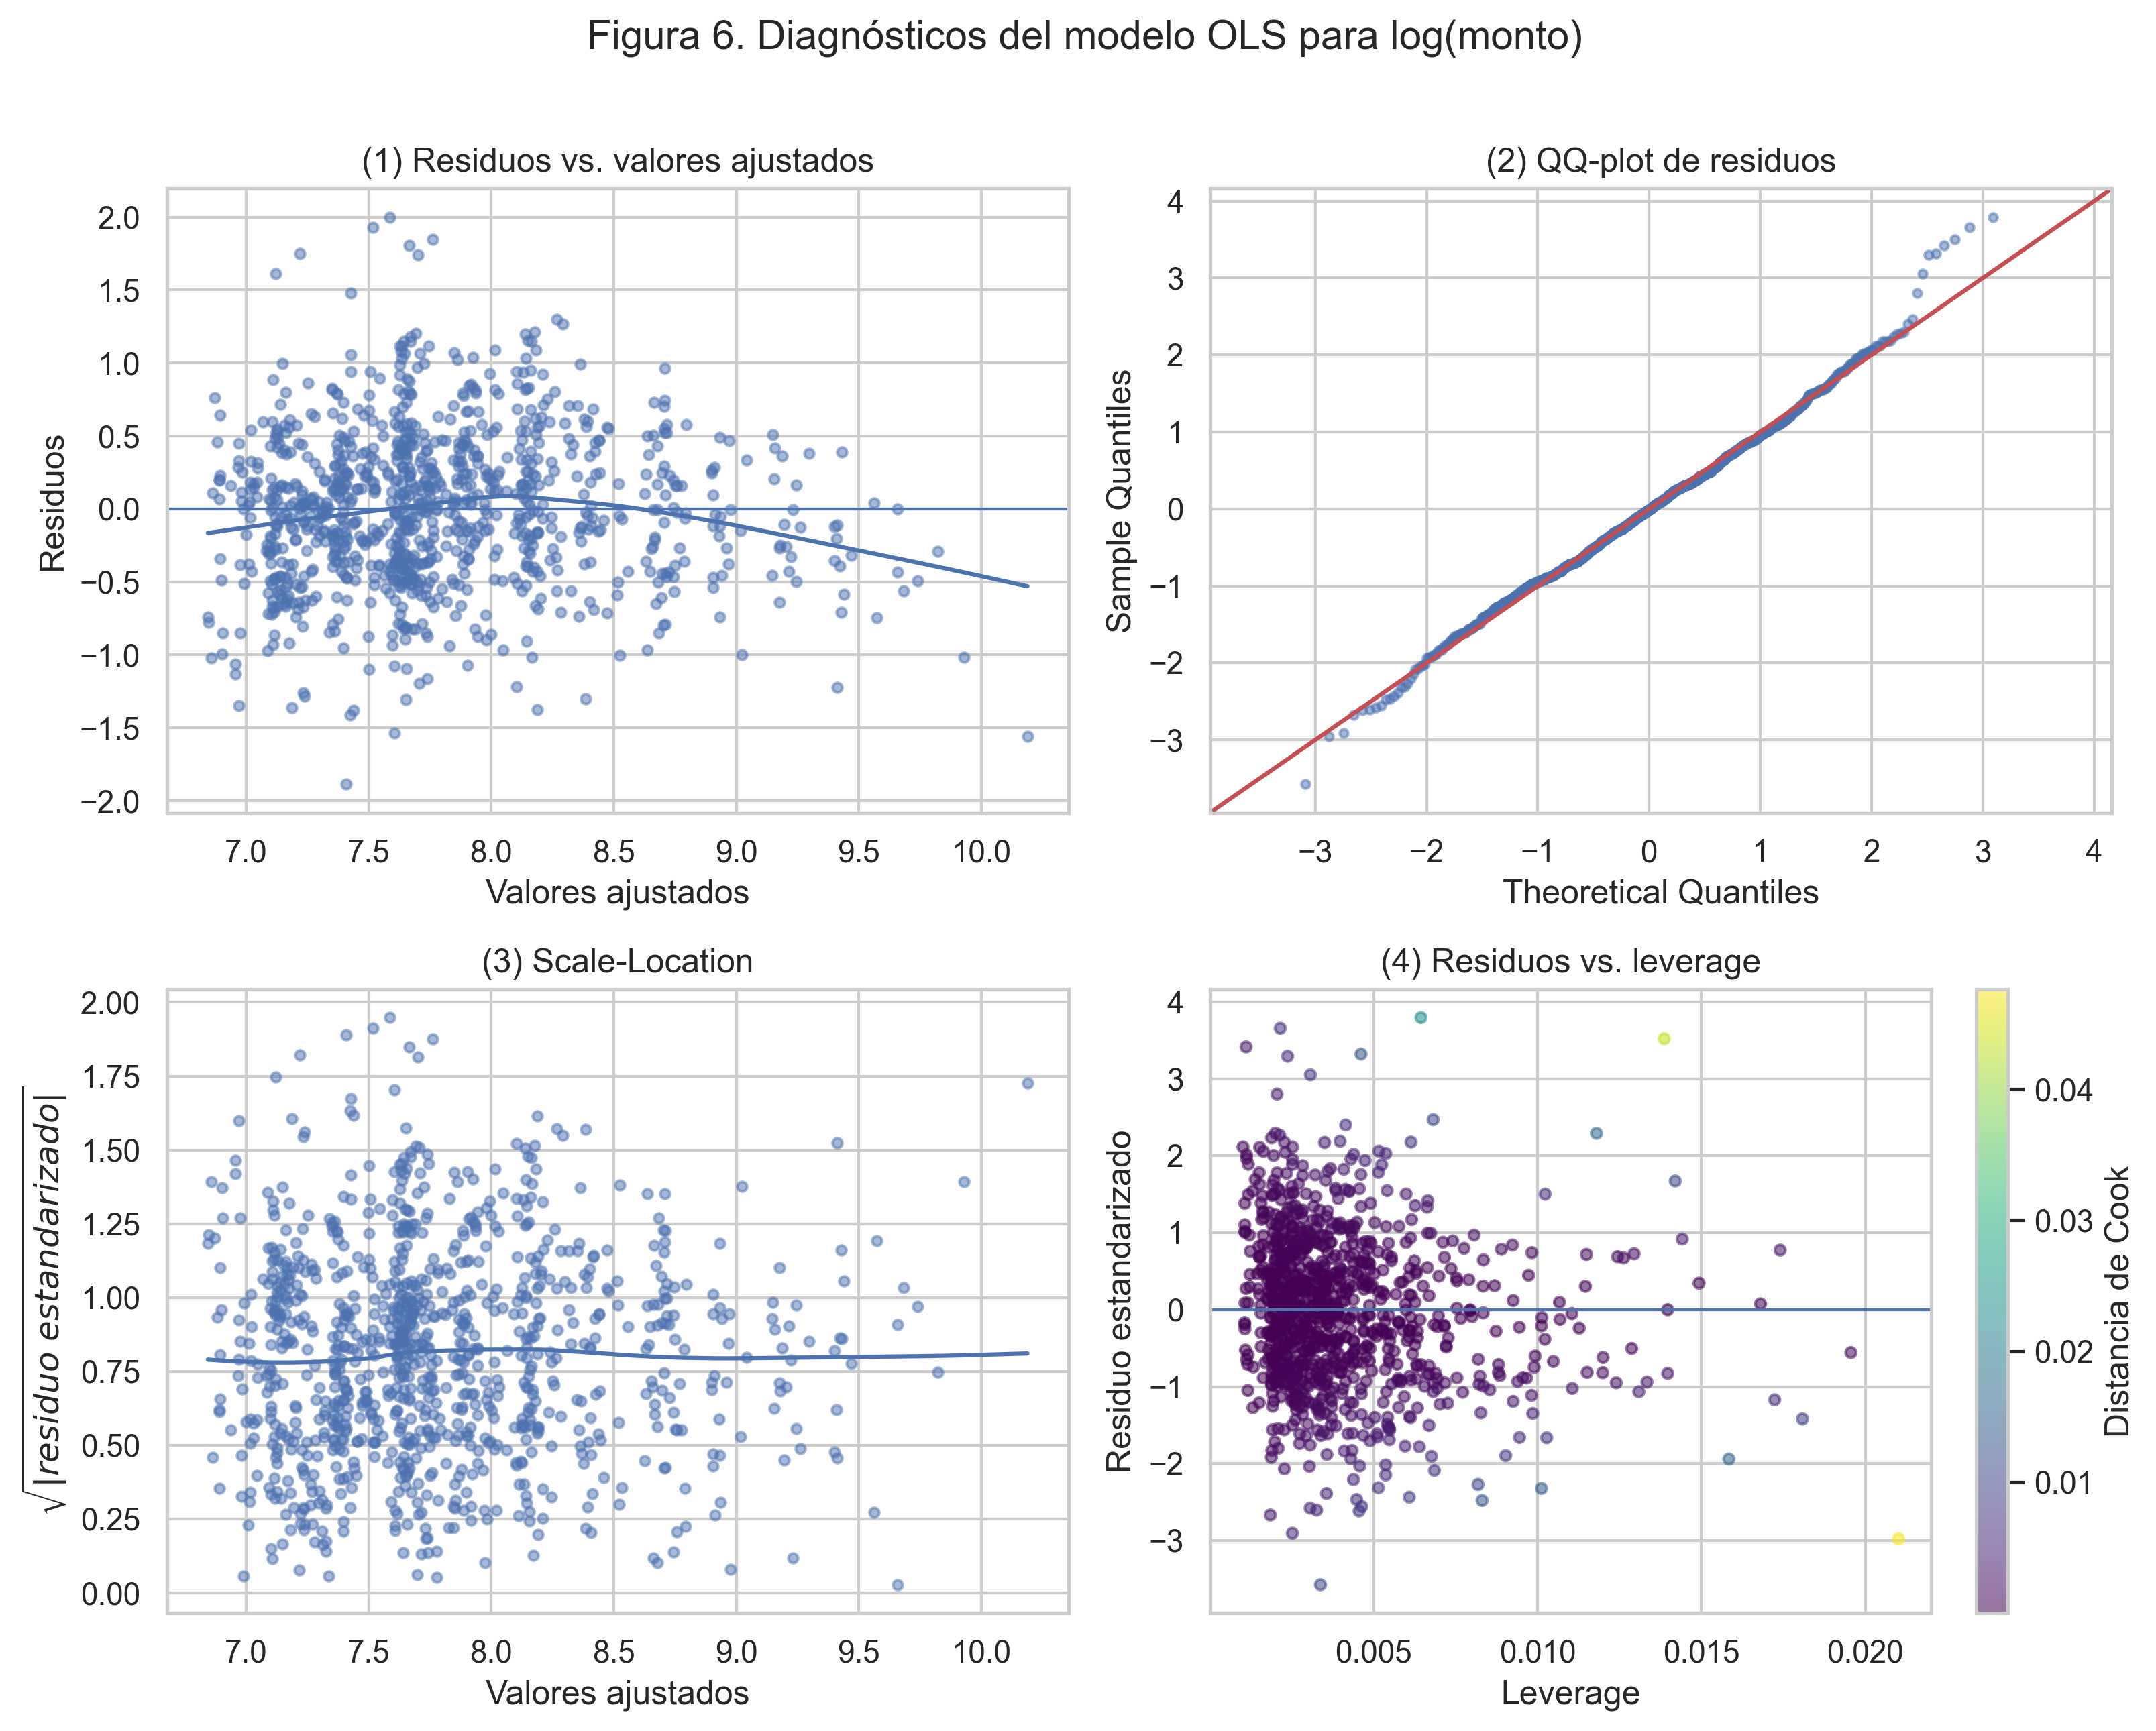
\includegraphics[
        width=\textwidth
    ]{
        figura_06_diagnosticos_modelo_ols.png
    }

    \caption{
        Diagnósticos del modelo OLS para
        \(\log(\variable{monto})\): residuos frente a valores ajustados,
        gráfico Q--Q, gráfico Scale--Location y residuos estandarizados
        frente a leverage.
    }

    \label{fig:diagnosticos-ols}
\end{figure}

El gráfico de residuos frente a valores ajustados no muestra una
curvatura dominante, aunque se observan pequeñas variaciones locales en
la línea suavizada. La dispersión alrededor de cero es razonablemente
estable.

El gráfico Q--Q presenta una alineación adecuada en la región central,
con desviaciones moderadas en las colas. Esto sugiere una aproximación
normal razonable para la mayor parte de los residuos, aunque no una
normalidad estricta.

El gráfico Scale--Location tampoco presenta una forma de embudo marcada.
La línea suavizada muestra variaciones leves, pero no una expansión
sistemática de la varianza a lo largo de los valores ajustados.

Finalmente, el gráfico de residuos frente a leverage permite identificar
observaciones que combinan valores poco habituales de los predictores con
residuos elevados. La distancia de Cook máxima fue:

\[
D_{\max}=\num{0.0476}.
\]

Utilizando el umbral exploratorio:

\[
\frac{4}{n}
=
\frac{4}{1000}
=
0.004,
\]

se identificaron \(52\) observaciones por encima de dicho valor. Este
umbral es deliberadamente sensible y funciona como una señal para
revisión, no como una regla automática de exclusión.

La distancia máxima permanece muy por debajo de uno, por lo que no se
observa una única operación con influencia extrema sobre el ajuste.
Las observaciones señaladas se conservaron porque corresponden a
registros válidos y su eliminación no estaba justificada por un error
documentado.

\subsection{Normalidad de los residuos}

La normalidad se evaluó formalmente mediante la prueba de Shapiro--Wilk:

\[
H_0:
\text{los residuos siguen una distribución normal},
\]

\[
H_1:
\text{los residuos no siguen una distribución normal}.
\]

El resultado fue:

\[
W=\num{0.9951},
\qquad
p=\num{0.00275}.
\]

Al nivel de significancia de \(0.05\), se rechaza la normalidad estricta.
Sin embargo, el valor de \(W\) es cercano a uno y el gráfico Q--Q muestra
que las principales desviaciones se concentran en las colas.

Con \(n=1000\), las pruebas de normalidad tienen capacidad para detectar
desviaciones pequeñas que no necesariamente producen un deterioro
práctico importante de la inferencia. Por esta razón, el resultado se
interpreta junto con los gráficos, el tamaño de la muestra y la
comparación posterior de los errores estándar clásicos y robustos.

\subsection{Homocedasticidad: prueba de Breusch--Pagan}

La constancia de la varianza se evaluó mediante:

\[
H_0:
\operatorname{Var}(\varepsilon_i\mid X_i)=\sigma^2,
\]

\[
H_1:
\operatorname{Var}(\varepsilon_i\mid X_i)
\text{ no es constante}.
\]

La prueba de Breusch--Pagan produjo:

\[
LM=\num{5.888},
\qquad
p=\num{0.11716},
\]

y la versión basada en \(F\):

\[
F=\num{1.967},
\qquad
p=\num{0.11733}.
\]

Como ambos valores \(p\) son superiores a \(0.05\), no se rechaza la
hipótesis de varianza constante. La homocedasticidad constituye una
aproximación razonable para esta especificación.

No rechazar \(H_0\) no demuestra que la varianza sea exactamente
constante. Indica que el test no encontró evidencia suficiente de
heterocedasticidad con los datos y la forma funcional utilizadas.

\subsection{Inferencia robusta HC3}

Como comprobación de sensibilidad, se recalcularon los errores estándar
mediante el estimador robusto HC3. Esta corrección mantiene los
coeficientes y predicciones, pero modifica la matriz de covarianza
utilizada en la inferencia.

\begin{table}[H]
    \centering
    \caption{Comparación entre la inferencia clásica y la corrección
    robusta HC3.}
    \label{tab:hc3-ols}

    \begin{tabular}{
        @{}
        l
        r
        r
        r
        r
        @{}
    }
        \toprule
        Variable
        & Coeficiente
        & EE clásico
        & EE HC3
        & \(p\) HC3 \\
        \midrule

        Intercepto
        & \num{7.4860}
        & \num{0.0742}
        & \num{0.0748}
        & \(<0.001\) \\

        Duración
        & \num{0.0431}
        & \num{0.0014}
        & \num{0.0015}
        & \(<0.001\) \\

        Tasa de la cuota
        & \num{-0.2476}
        & \num{0.0150}
        & \num{0.0156}
        & \(<0.001\) \\

        Edad
        & \num{0.0039}
        & \num{0.0015}
        & \num{0.0016}
        & \num{0.0144} \\

        \bottomrule
    \end{tabular}
\end{table}

Los errores HC3 son ligeramente mayores, pero las conclusiones no
cambian. Duración, tasa de la cuota y edad mantienen asociaciones
estadísticamente significativas.

La estabilidad frente a HC3 respalda que los resultados no dependen
exclusivamente de la matriz de covarianza clásica. La edad continúa
siendo significativa, aunque con menor evidencia que las otras dos
variables.

\subsection{Validación cruzada de cinco particiones}

La capacidad de generalización se evaluó mediante validación cruzada
\(k\)-fold con:

\[
k=5.
\]

La muestra se dividió aleatoriamente en cinco grupos. En cada iteración,
cuatro particiones se utilizaron para ajustar el modelo y la restante
para evaluarlo. La semilla utilizada fue \(\texttt{SEED}=2026\).

El desempeño se midió mediante \(R^2\) y RMSE en la escala de
\(\log(\variable{monto})\).

\begin{table}[H]
    \centering
    \caption{Resultados de validación cruzada del modelo OLS.}
    \label{tab:cv-ols}

    \begin{tabular}{ccc}
        \toprule
        Partición & \(R^2\) & RMSE \\
        \midrule
        1 & \num{0.5321} & \num{0.5776} \\
        2 & \num{0.4972} & \num{0.5292} \\
        3 & \num{0.5943} & \num{0.4959} \\
        4 & \num{0.5439} & \num{0.4861} \\
        5 & \num{0.4901} & \num{0.5561} \\
        \midrule
        Media & \num{0.5315} & \num{0.5290} \\
        Desviación estándar de \(R^2\)
        & \num{0.0418}
        & --- \\
        \bottomrule
    \end{tabular}
\end{table}

El \(R^2\) medio fuera de muestra fue:

\[
\overline{R^2}_{\mathrm{CV}}
=
\num{0.5315}
\pm
\num{0.0418}.
\]

El RMSE medio fue:

\[
\operatorname{RMSE}_{\mathrm{CV}}
=
\num{0.5290}
\]

en la escala logarítmica.

El desempeño de validación es muy próximo al obtenido con la muestra
completa:

\[
R^2_{\mathrm{completo}}=\num{0.5379}.
\]

La diferencia entre ambos valores es reducida, lo que indica que el
modelo mantiene una capacidad explicativa estable en observaciones no
utilizadas durante cada ajuste. No se observa evidencia importante de
sobreajuste dentro del esquema de validación aplicado.

\subsection{Conclusión del modelo lineal}

El modelo OLS proporciona una representación parsimoniosa e
interpretable de la estructura del monto. La duración, la carga de la
cuota y la edad explican conjuntamente cerca del \(54\,\%\) de la
variabilidad de su logaritmo.

La duración presenta la asociación positiva dominante. La tasa de la
cuota mantiene una asociación negativa importante y la edad aporta una
señal positiva pequeña. Los VIF cercanos a uno descartan problemas
relevantes de multicolinealidad entre los predictores seleccionados.

Los diagnósticos no muestran evidencia de heterocedasticidad y la
inferencia robusta HC3 conserva las conclusiones. La prueba de
Shapiro--Wilk detecta una desviación respecto de la normalidad estricta,
pero el comportamiento gráfico, el tamaño de la muestra y la estabilidad
de los errores robustos indican que dicha desviación no modifica de forma
sustantiva la lectura del modelo.

Finalmente, la validación cruzada muestra un desempeño cercano al ajuste
completo. El modelo es útil para comprender la relación entre el plazo,
la capacidad de pago aproximada, la edad y el monto otorgado.

No obstante, este resultado no responde todavía qué solicitantes tienen
mayor probabilidad de mal crédito. Esa pregunta requiere un modelo con
respuesta binaria, desarrollado en el bloque siguiente mediante
regresión logística.

\subsection{Regresión logística para la probabilidad de mal crédito}
\label{subsec:logit}

La segunda parte del modelamiento utiliza como respuesta la variable:

\[
Y_i=\variable{mal_credito}_i,
\]

donde:

\[
Y_i=
\begin{cases}
1, & \text{si el registro corresponde a mal riesgo},\\
0, & \text{si corresponde a buen riesgo}.
\end{cases}
\]

Sea:

\[
p_i
=
\Pr(Y_i=1\mid\mathbf{x}_i)
\]

la probabilidad condicional de que la observación \(i\) sea clasificada
como mal crédito. La regresión logística relaciona esta probabilidad con
los predictores mediante:

\[
\operatorname{logit}(p_i)
=
\log\left(
    \frac{p_i}{1-p_i}
\right)
=
\beta_0+\mathbf{x}_i^{\mathsf{T}}\boldsymbol{\beta}.
\]

De forma equivalente:

\[
p_i
=
\frac{
    \exp\left(
        \beta_0+\mathbf{x}_i^{\mathsf{T}}\boldsymbol{\beta}
    \right)
}{
    1+
    \exp\left(
        \beta_0+\mathbf{x}_i^{\mathsf{T}}\boldsymbol{\beta}
    \right)
}.
\]

El modelo estima probabilidades individuales de mal riesgo. La
transformación de esas probabilidades en una decisión binaria requiere
un umbral, cuya selección se analiza posteriormente.

\subsubsection{Diseño de entrenamiento y prueba}

El conjunto de datos se dividió de forma estratificada en:

\[
70\,\% \text{ para entrenamiento}
\qquad\text{y}\qquad
30\,\% \text{ para prueba}.
\]

La partición resultante fue:

\[
n_{\mathrm{train}}=700,
\qquad
n_{\mathrm{test}}=300.
\]

La tasa de mal crédito se mantuvo en \(30.0\,\%\) en ambos subconjuntos.
Por tanto, el conjunto de entrenamiento contiene \(210\) malos créditos
y el conjunto de prueba contiene \(90\).

La estratificación permite comparar el desempeño sin que una variación
accidental de la prevalencia modifique de manera importante las métricas.
El modelo se ajustó exclusivamente con el conjunto de entrenamiento. El
conjunto de prueba permaneció separado hasta la evaluación final.

La semilla utilizada fue:

\[
\texttt{SEED}=2026.
\]

\subsubsection{Especificación del modelo}

La especificación incorporó variables contractuales, antecedentes
crediticios y señales de estabilidad financiera:

\[
\begin{aligned}
\operatorname{logit}(p_i)
={}&
\beta_0
+\beta_1\variable{duracion}_i
+\beta_2\variable{log_monto}_i
+\beta_3\variable{tasa_cuota}_i
+\beta_4\variable{edad}_i\\
&+\text{estado de cuenta}
+\text{historial crediticio}
+\text{ahorros}\\
&+\text{antigüedad laboral}
+\text{vivienda}
+\text{otros planes de pago}.
\end{aligned}
\]

Las variables categóricas se introdujeron mediante indicadores, dejando
una categoría de referencia en cada grupo. Las referencias fueron:

\begin{itemize}
    \item estado de cuenta: \texttt{A11}, saldo menor que cero;

    \item historial crediticio: \texttt{A30}, sin créditos previos o
    todos pagados;

    \item ahorros: \texttt{A61}, menos de \(100\) DM;

    \item empleo actual: \texttt{A71}, desempleado;

    \item vivienda: \texttt{A151}, alquilada;

    \item otros planes de pago: \texttt{A141}, banco.
\end{itemize}

Los coeficientes se estimaron mediante máxima verosimilitud con
\texttt{statsmodels}. El algoritmo convergió correctamente y el modelo
contiene \(24\) coeficientes, incluido el intercepto.

El pseudo-\(R^2\) de McFadden en entrenamiento fue:

\[
R^2_{\mathrm{McFadden}}
=
0.2202.
\]

Este valor no debe interpretarse como el porcentaje de variabilidad
explicada y no es comparable directamente con el \(R^2\) de una
regresión OLS. Se utiliza como una medida relativa de mejora frente a un
modelo que solo contiene intercepto.

\subsection{Interpretación mediante odds ratios}

En una regresión logística, el coeficiente \(\beta_j\) representa un
cambio en el logaritmo de las \textit{odds}. Para facilitar la
interpretación se utiliza:

\[
\OR_j
=
\exp(\beta_j).
\]

Cuando \(\OR_j>1\), las \textit{odds} de mal crédito aumentan. Cuando
\(\OR_j<1\), disminuyen. En ambos casos, la comparación mantiene
constantes los demás predictores del modelo.

Es importante distinguir \textit{odds} de probabilidad. Un aumento del
\(20\,\%\) en las \textit{odds} no equivale necesariamente a un aumento
de veinte puntos porcentuales en la probabilidad, porque el efecto sobre
la probabilidad depende de su nivel inicial.

\subsubsection{Predictores numéricos}

La Tabla~\ref{tab:or-numericos} presenta los resultados de los
predictores numéricos.

\begin{table}[H]
    \centering
    \caption{Odds ratios de los predictores numéricos del modelo
    logístico.}
    \label{tab:or-numericos}

    \begin{tabular}{
        @{}
        l
        r
        c
        r
        @{}
    }
        \toprule
        Predictor
        & OR
        & IC del \(95\,\%\)
        & \(p\) \\
        \midrule

        Duración
        & \num{1.0390}
        & \([1.0160,\;1.0625]\)
        & \num{0.0008} \\

        Logaritmo del monto
        & \num{1.0658}
        & \([0.7483,\;1.5181]\)
        & \num{0.7238} \\

        Tasa de la cuota
        & \num{1.2283}
        & \([1.0085,\;1.4959]\)
        & \num{0.0409} \\

        Edad
        & \num{0.9972}
        & \([0.9775,\;1.0172]\)
        & \num{0.7798} \\

        \bottomrule
    \end{tabular}
\end{table}

Manteniendo constantes las demás variables, cada mes adicional de
duración se asocia con un aumento aproximado del \(3.9\,\%\) en las
\textit{odds} de mal crédito:

\[
100(1.0390-1)=3.9\,\%.
\]

El intervalo de confianza se mantiene por encima de uno y el valor
\(p\) es inferior a \(0.05\). La duración conserva, por tanto, una
asociación positiva después de controlar por las demás características.

Una unidad adicional en la escala de \variable{tasa_cuota} se asocia con
un incremento aproximado del \(22.8\,\%\) en las \textit{odds}. Esta
interpretación se refiere a un cambio entre niveles de una escala
ordinal, no a un incremento de un punto porcentual del ingreso.

En contraste, \variable{log_monto} deja de ser estadísticamente
significativo:

\[
\OR=1.0658,
\qquad
p=0.7238.
\]

El monto mostró una diferencia marginal entre buenos y malos créditos,
pero no aporta evidencia de una asociación independiente una vez que el
modelo incorpora duración, liquidez, historial y otras variables. Parte
de su señal inicial parece estar compartida con la duración del préstamo.

La edad tampoco presenta evidencia de una asociación condicional dentro
de esta especificación.

\subsubsection{Categorías con evidencia estadística}

La Tabla~\ref{tab:or-categoricos} resume las categorías cuyo intervalo
del \(95\,\%\) no contiene el valor uno.

\begin{table}[H]
    \centering
    \caption{Categorías con asociación estadísticamente significativa en
    el modelo logístico.}
    \label{tab:or-categoricos}

    \footnotesize
    \begin{tabularx}{\textwidth}{
        @{}
        >{\raggedright\arraybackslash}p{3.4cm}
        >{\raggedright\arraybackslash}p{4.1cm}
        >{\centering\arraybackslash}p{1.3cm}
        >{\centering\arraybackslash}p{2.5cm}
        >{\centering\arraybackslash}p{1.4cm}
        @{}
    }
        \toprule
        Variable
        & Categoría frente a referencia
        & OR
        & IC del \(95\,\%\)
        & \(p\) \\
        \midrule

        Ahorros
        & \texttt{A64}: \(1000\) DM o más
          frente a \texttt{A61}
        & \num{0.1617}
        & \([0.0349,\;0.7495]\)
        & \num{0.0199} \\

        Estado de cuenta
        & \texttt{A14}: sin cuenta corriente
          frente a \texttt{A11}
        & \num{0.1803}
        & \([0.1079,\;0.3014]\)
        & \(<0.001\) \\

        Historial crediticio
        & \texttt{A34}: cuenta crítica u otros créditos
          frente a \texttt{A30}
        & \num{0.2413}
        & \([0.0910,\;0.6403]\)
        & \num{0.0043} \\

        Estado de cuenta
        & \texttt{A13}: saldo de \(200\) DM o más
          frente a \texttt{A11}
        & \num{0.3121}
        & \([0.1384,\;0.7038]\)
        & \num{0.0050} \\

        Empleo actual
        & \texttt{A74}: entre cuatro y siete años
          frente a \texttt{A71}
        & \num{0.4037}
        & \([0.1632,\;0.9987]\)
        & \num{0.0497} \\

        Ahorros
        & \texttt{A65}: desconocido o sin cuenta
          frente a \texttt{A61}
        & \num{0.4303}
        & \([0.2421,\;0.7647]\)
        & \num{0.0041} \\

        Vivienda
        & \texttt{A152}: propia
          frente a \texttt{A151}
        & \num{0.5868}
        & \([0.3552,\;0.9694]\)
        & \num{0.0374} \\

        Estado de cuenta
        & \texttt{A12}: saldo entre \(0\) y \(200\) DM
          frente a \texttt{A11}
        & \num{0.6041}
        & \([0.3776,\;0.9665]\)
        & \num{0.0355} \\

        \bottomrule
    \end{tabularx}
\end{table}

El estado de la cuenta corriente presenta un gradiente coherente respecto
de la categoría de saldo negativo. Los perfiles con saldo positivo y los
registros sin una cuenta corriente codificada muestran menores
\textit{odds} que el grupo de referencia.

El resultado de \texttt{A14} no implica que carecer de cuenta corriente
sea, en términos generales, una condición financiera favorable. La
comparación se realiza específicamente frente a solicitantes con saldo
negativo. Además, la categoría histórica puede condensar perfiles
heterogéneos que no pueden separarse con la documentación disponible.

Los niveles altos de ahorro presentan menores \textit{odds} que el grupo
con menos de \(100\) DM. La categoría \texttt{A65} combina ausencia de
cuenta e información desconocida, por lo que su asociación debe
interpretarse con cautela.

La vivienda propia también se asocia con menores \textit{odds} frente a
la vivienda alquilada. La antigüedad laboral de cuatro a siete años
presenta una asociación protectora, aunque su valor \(p=0.0497\) y el
límite superior del intervalo, próximo a uno, indican evidencia débil y
sensible al redondeo.

El resultado del historial \texttt{A34} debe leerse únicamente como un
contraste condicional respecto de \texttt{A30}. La denominación histórica
de las categorías no permite convertir directamente ese coeficiente en
una regla general de aprobación.

\begin{figure}[H]
    \centering

    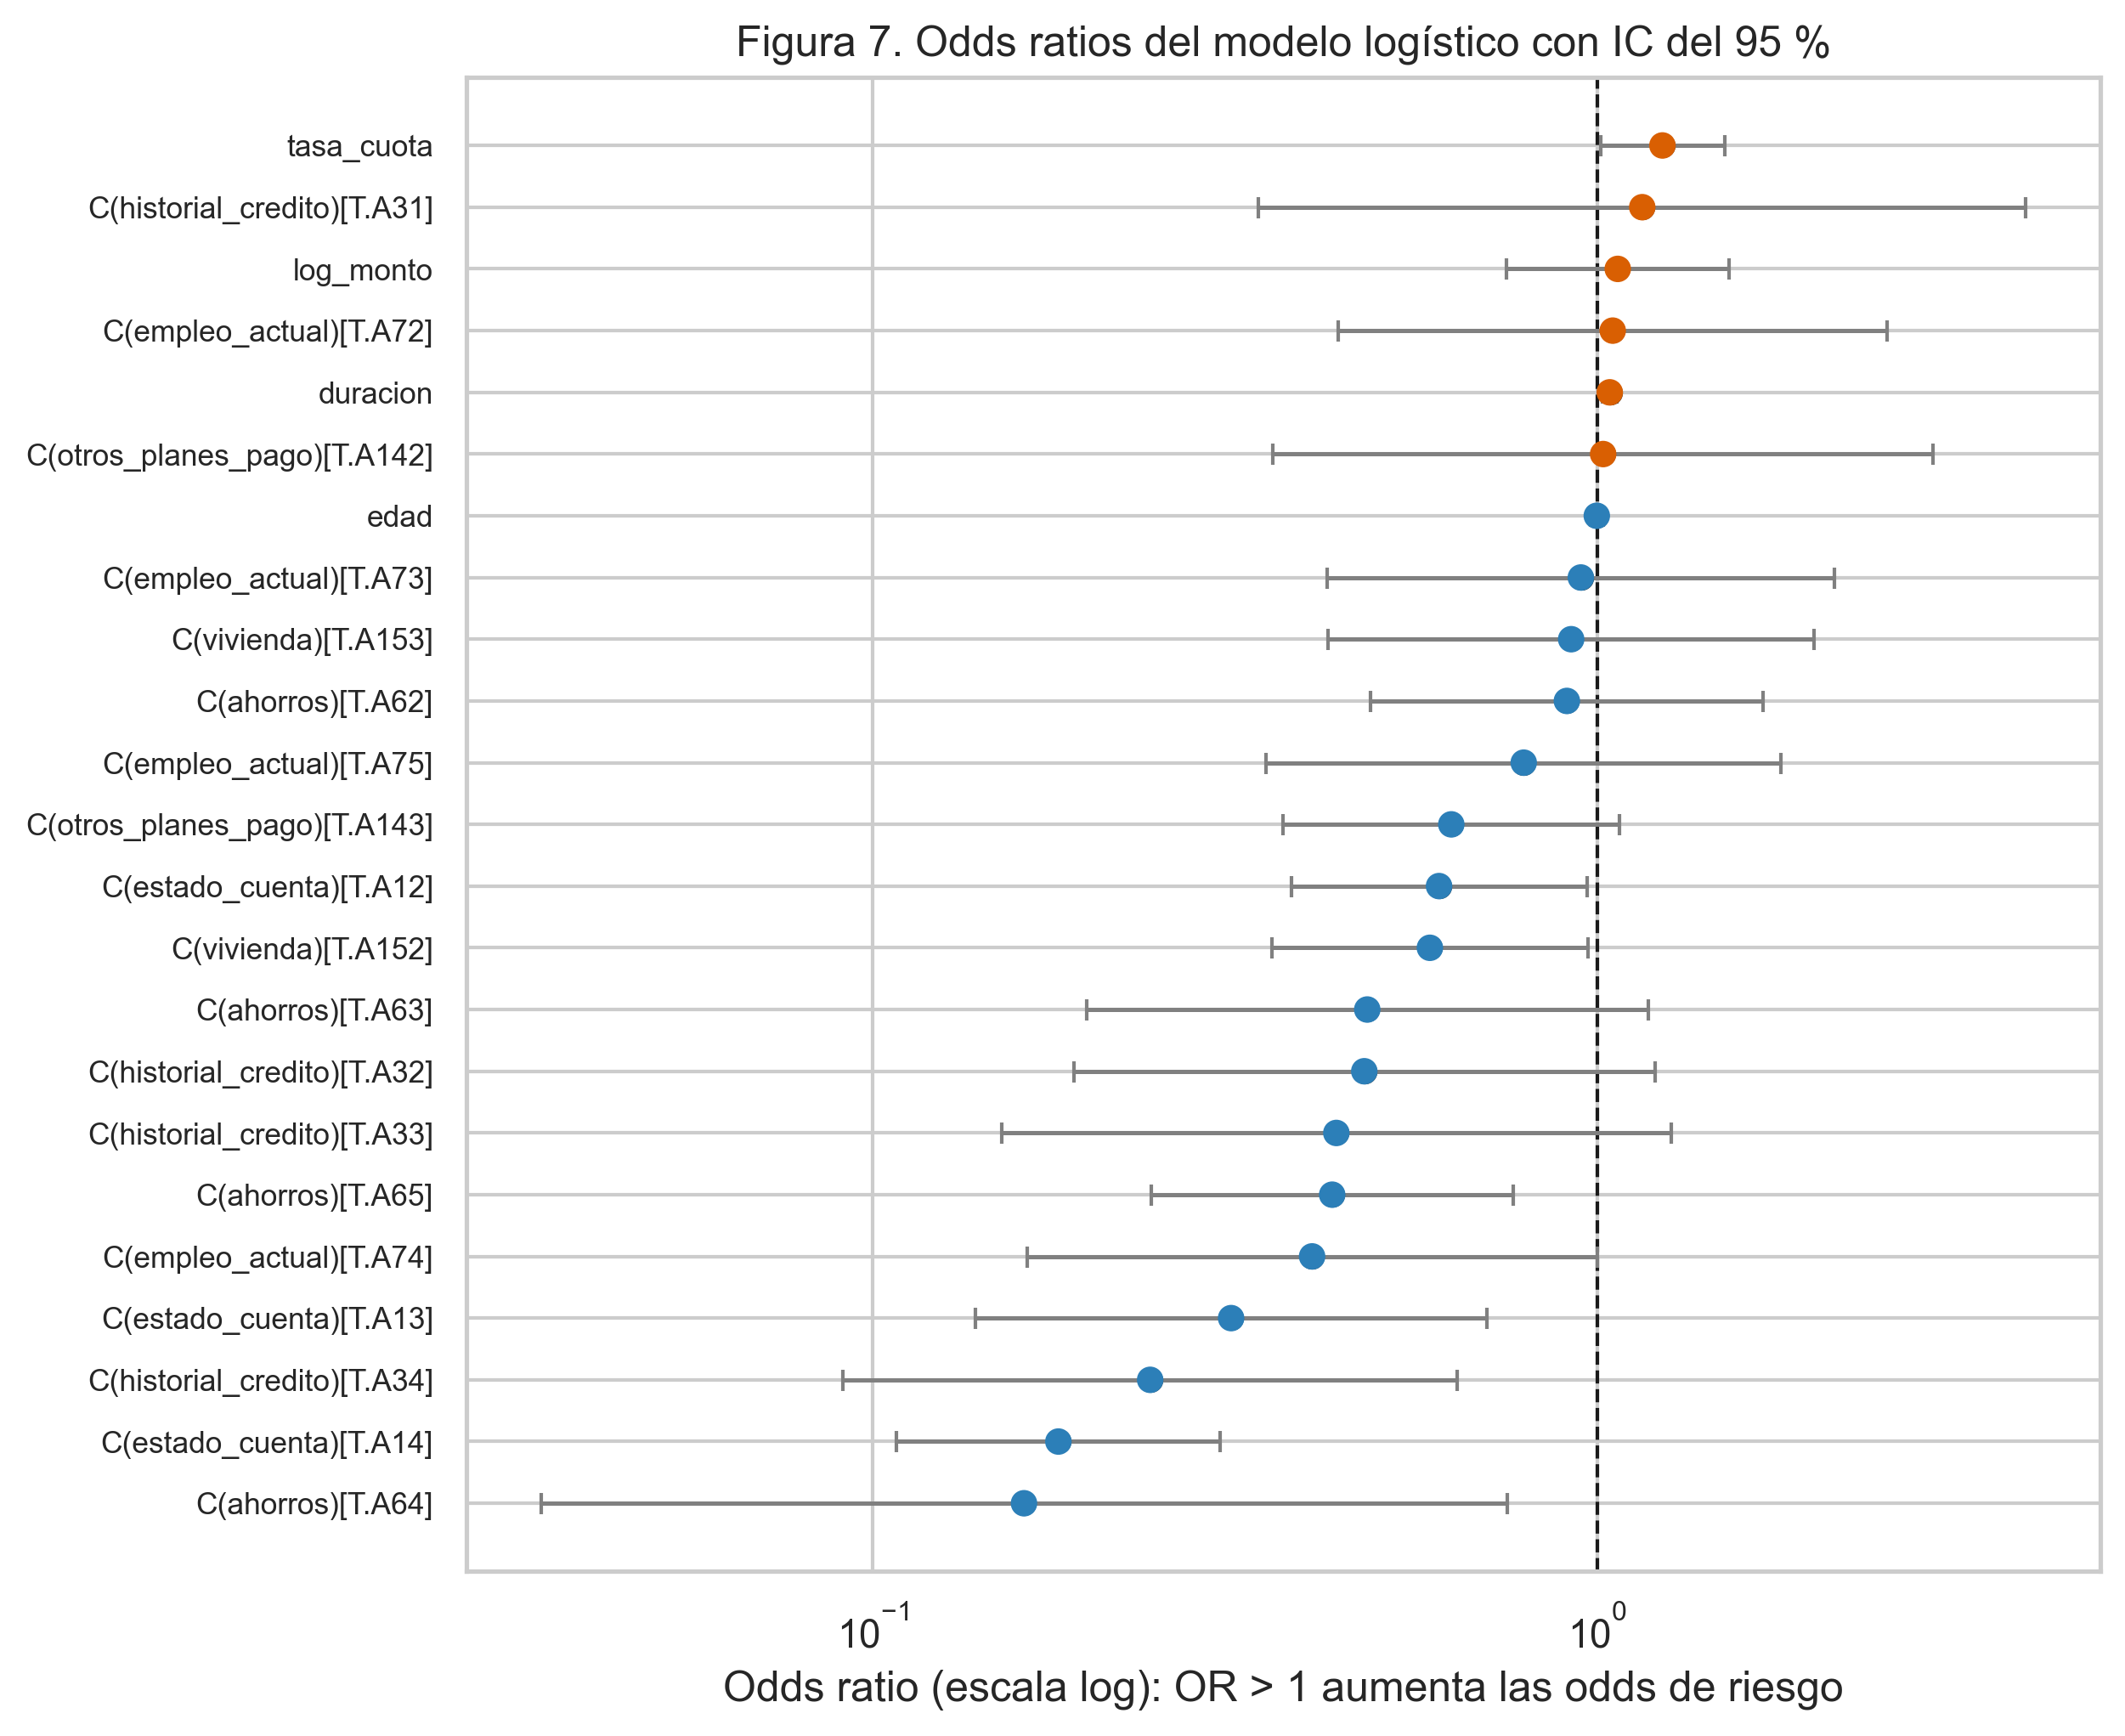
\includegraphics[
        width=0.92\textwidth
    ]{
        figura_07_odds_ratios_modelo_logistico.png
    }

    \caption{
        Odds ratios e intervalos de confianza del \(95\,\%\) del modelo
        logístico. La línea vertical representa ausencia de asociación
        en la escala de odds ratios.
    }

    \label{fig:odds-ratios-logit}
\end{figure}

La Figura~\ref{fig:odds-ratios-logit} muestra simultáneamente la magnitud,
dirección e incertidumbre de todos los términos. Los intervalos amplios
de algunas categorías reflejan tamaños de grupo reducidos y menor
precisión.

\begin{hallazgo}
La duración mantiene la asociación numérica más consistente con el mal
crédito. El estado de cuenta, los ahorros, el historial, la vivienda y
la carga de la cuota también aportan información condicional. El monto
pierde significancia al controlar por estas variables.
\end{hallazgo}

\subsection{Capacidad discriminativa}

La calidad de un modelo de riesgo no se resume en sus coeficientes. Es
necesario evaluar si las probabilidades estimadas ordenan adecuadamente
los casos de buen y mal crédito en observaciones no utilizadas durante
el ajuste.

La métrica principal independiente del umbral fue el área bajo la curva
ROC:

\[
\AUC_{\mathrm{test}}
=
0.7740.
\]

Este valor puede interpretarse como la probabilidad de que, al elegir al
azar un mal crédito y un buen crédito del conjunto de prueba, el modelo
asigne una puntuación de riesgo mayor al primero.

El resultado indica una capacidad discriminativa claramente superior al
azar, aunque lejos de una separación perfecta. Persisten buenos y malos
créditos con probabilidades similares.

También se calculó el estadístico de Kolmogorov--Smirnov utilizado en
\textit{credit scoring}:

\[
KS
=
\max_t
\left[
    \operatorname{TPR}(t)
    -
    \operatorname{FPR}(t)
\right].
\]

El resultado fue:

\[
KS=0.4810,
\]

alcanzado alrededor del umbral:

\[
t=0.369.
\]

Este resultado muestra una separación apreciable entre las distribuciones
de puntajes de ambas clases. Sin embargo, el umbral que maximiza KS no
tiene por qué minimizar el costo económico de clasificación.

La AUC evalúa capacidad de ordenamiento. No informa por sí sola si las
probabilidades están calibradas, cuál es la rentabilidad de la política
crediticia ni qué umbral debe utilizarse.

\subsection{Validación cruzada del modelo logístico}

La estabilidad se examinó mediante validación cruzada estratificada de
cinco particiones. Dentro de cada partición, las variables categóricas se
codificaron mediante indicadores y las numéricas se estandarizaron usando
exclusivamente la información del conjunto de entrenamiento
correspondiente.

Esta construcción evita que el preprocesamiento utilice información de
la partición de validación.

Los resultados fueron:

\begin{table}[H]
    \centering
    \caption{ROC--AUC por partición en la validación cruzada del modelo
    logístico.}
    \label{tab:cv-logit}

    \begin{tabular}{cc}
        \toprule
        Partición & ROC--AUC \\
        \midrule
        1 & \num{0.7785} \\
        2 & \num{0.7744} \\
        3 & \num{0.8013} \\
        4 & \num{0.7485} \\
        5 & \num{0.7399} \\
        \midrule
        Media & \num{0.7685} \\
        Desviación estándar & \num{0.0221} \\
        \bottomrule
    \end{tabular}
\end{table}

La media de validación fue:

\[
\overline{\AUC}_{\mathrm{CV}}
=
0.7685
\pm
0.0221.
\]

La proximidad entre la AUC de prueba y la media de validación cruzada:

\[
0.7740
\approx
0.7685
\]

indica un desempeño estable entre particiones. No se observa una brecha
importante que sugiera sobreajuste bajo el diseño de evaluación
utilizado.

\subsection{Clasificación con el umbral estándar}

El umbral convencional clasifica una observación como mal riesgo cuando:

\[
\widehat{p}_i
\geq
0.50.
\]

Con este umbral, la matriz de confusión del conjunto de prueba fue:

\[
\begin{array}{c|cc}
 & \text{Predicho bueno} & \text{Predicho malo} \\
\hline
\text{Real bueno} & 180 & 30 \\
\text{Real malo}  & 48  & 42
\end{array}
\]

Por tanto:

\[
TN=180,
\quad
FP=30,
\quad
FN=48,
\quad
TP=42.
\]

Las métricas fueron:

\[
\operatorname{accuracy}
=
0.7400,
\]

\[
\operatorname{precision}
=
0.5833,
\]

\[
\operatorname{recall}
=
0.4667,
\]

\[
F_1
=
0.5185,
\]

\[
\operatorname{especificidad}
=
\frac{180}{180+30}
=
0.8571.
\]

Aunque la exactitud alcanza el \(74.0\,\%\), el modelo identifica menos
de la mitad de los malos créditos. De los \(90\) casos de mal riesgo,
\(48\) serían clasificados como buenos.

Este resultado ilustra por qué la exactitud no puede utilizarse como
único criterio: la política favorece la especificidad, pero conserva
demasiados falsos negativos para una matriz de costos que penaliza ese
error cinco veces más.

\subsection{Selección del umbral bajo costos asimétricos}

La matriz de costos asigna:

\[
C_{\mathrm{FN}}=5,
\qquad
C_{\mathrm{FP}}=1.
\]

Para una observación con probabilidad estimada \(p\), el costo esperado
de clasificarla como buen riesgo es:

\[
C(\text{predecir bueno})
=
C_{\mathrm{FN}}p.
\]

El costo esperado de clasificarla como mal riesgo es:

\[
C(\text{predecir malo})
=
C_{\mathrm{FP}}(1-p).
\]

La decisión de menor costo clasifica como mal riesgo cuando:

\[
C_{\mathrm{FP}}(1-p)
\leq
C_{\mathrm{FN}}p.
\]

Al despejar \(p\):

\[
p
\geq
\frac{
    C_{\mathrm{FP}}
}{
    C_{\mathrm{FP}}+C_{\mathrm{FN}}
}.
\]

Por tanto, el umbral teórico es:

\[
t^{*}
=
\frac{1}{1+5}
=
\frac{1}{6}
\approx
0.1667.
\]

Esta regla supone que los costos representan adecuadamente el problema y
que las probabilidades producidas por el modelo están razonablemente
calibradas. La AUC por sí sola no permite comprobar esta segunda
condición.

El umbral se deriva de la matriz de costos y no de la búsqueda del mejor
resultado en el conjunto de prueba. La curva empírica de costos se
utiliza únicamente como diagnóstico posterior.

\begin{figure}[H]
    \centering

    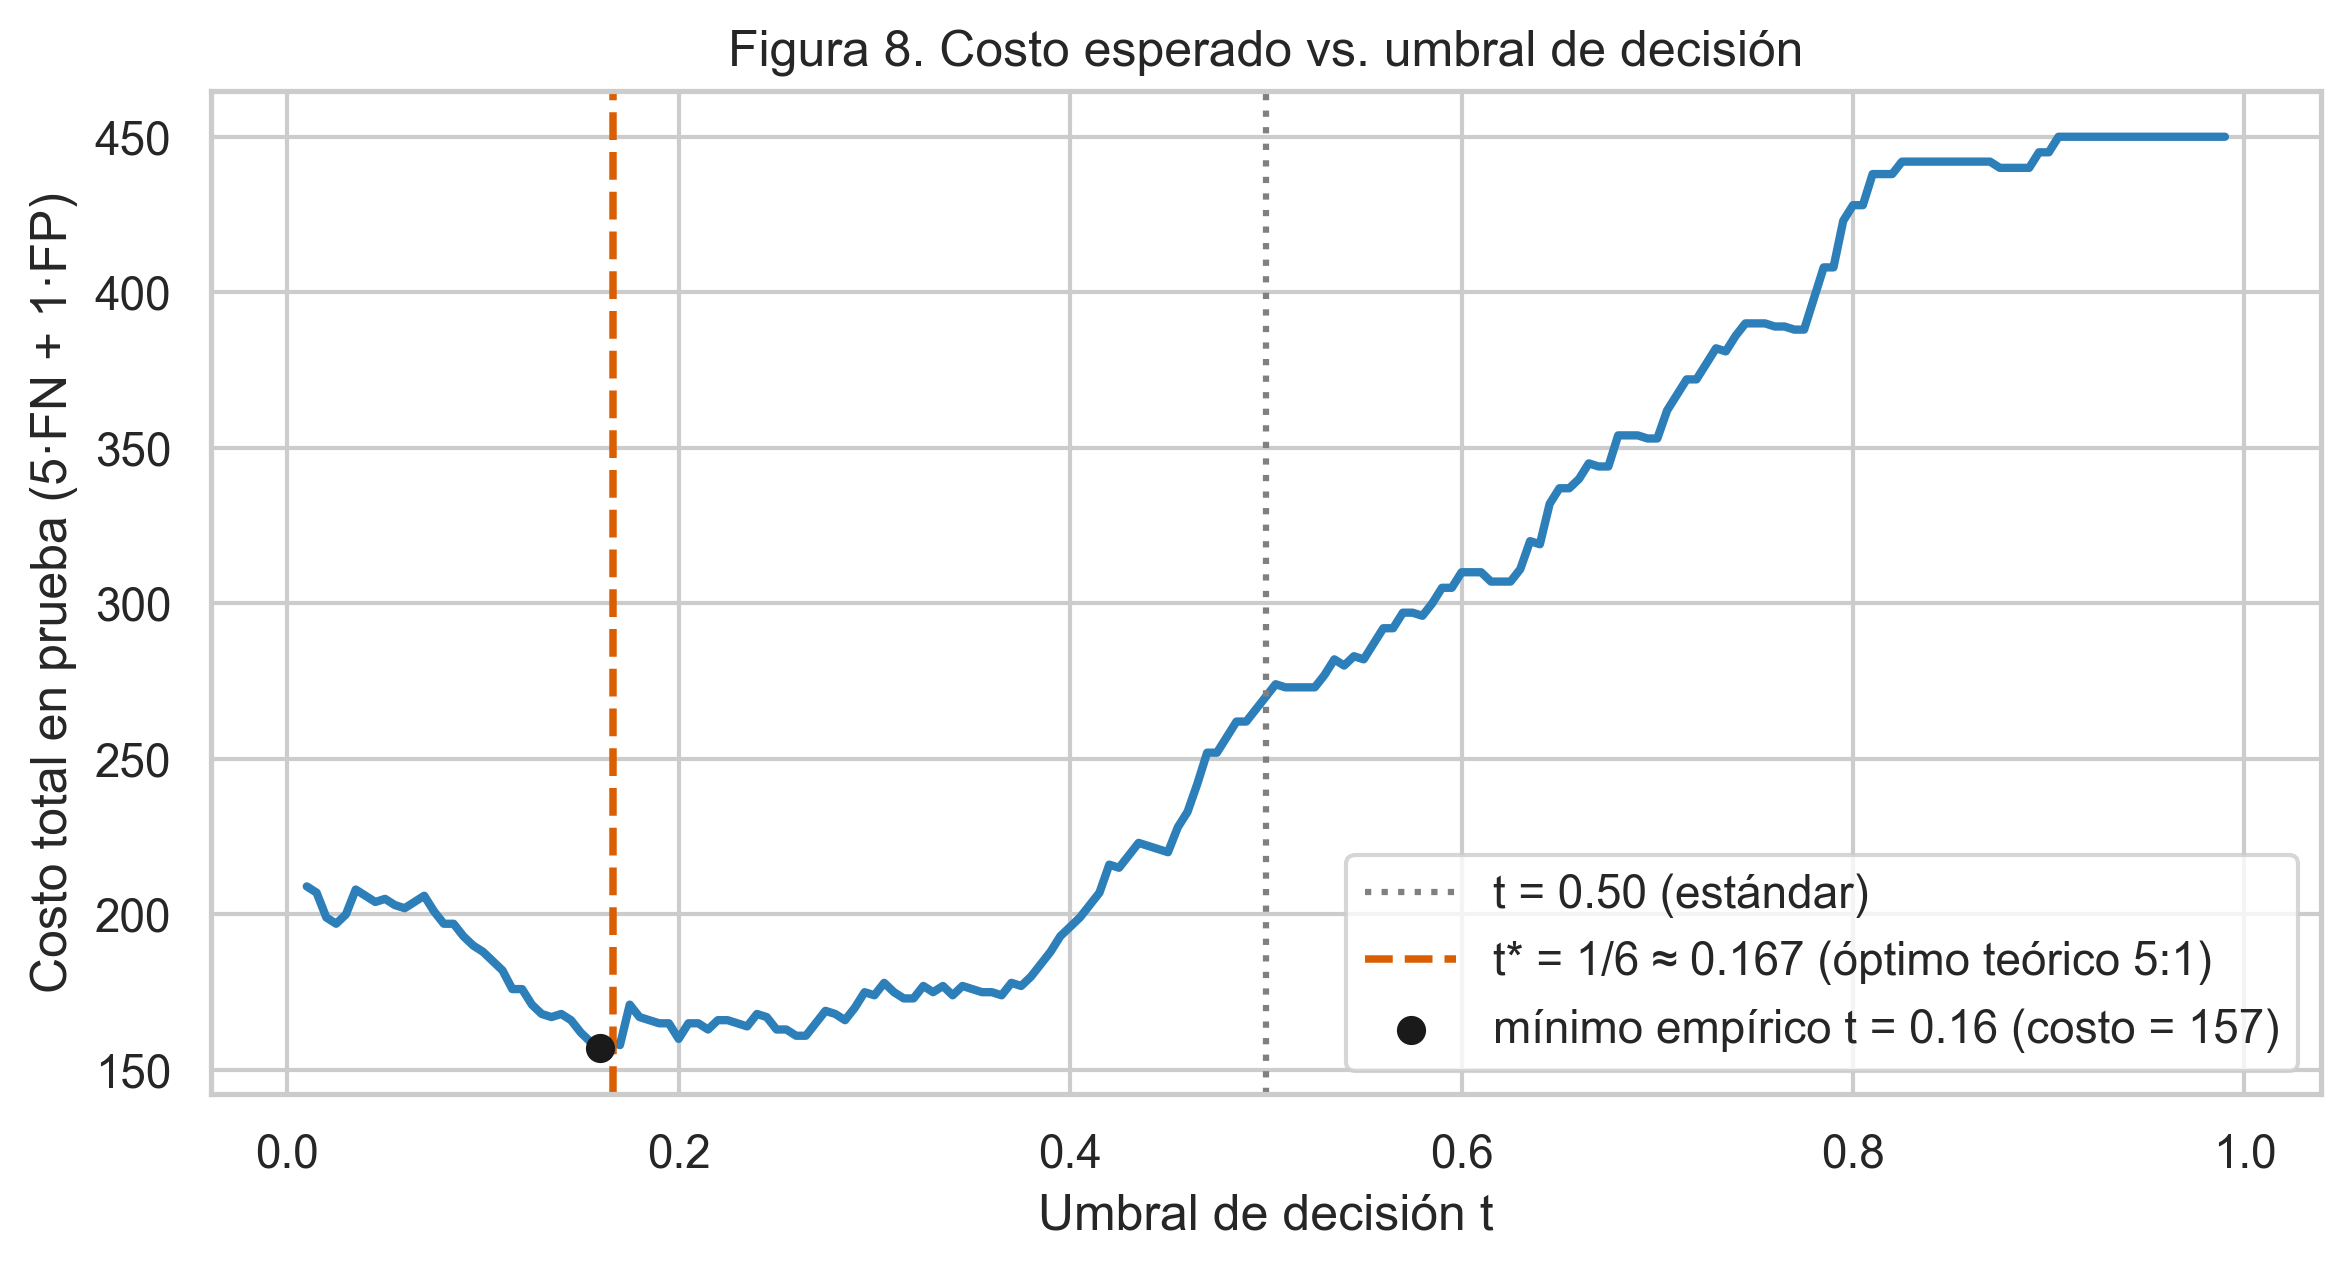
\includegraphics[
        width=0.88\textwidth
    ]{
        figura_08_costo_vs_umbral.png
    }

    \caption{
        Costo total de clasificación en el conjunto de prueba según el
        umbral. Se muestran el umbral estándar, el umbral teórico
        derivado de la matriz \(5:1\) y el mínimo empírico.
    }

    \label{fig:costo-umbral}
\end{figure}

El costo empírico mínimo se observa alrededor de:

\[
t_{\mathrm{emp}}=0.16,
\]

con un costo de \(157\) unidades. Este valor es prácticamente igual al
umbral teórico \(0.1667\), cuyo costo es \(158\). La diferencia de una
unidad no justifica reemplazar la regla derivada de costos por un umbral
optimizado sobre la misma muestra de prueba.

Seleccionar \(t_{\mathrm{emp}}\) como política final usando las etiquetas
del test introduciría optimismo. En un desarrollo real, cualquier ajuste
empírico del umbral debería efectuarse en validación y confirmarse sobre
un conjunto final independiente.

\subsection{Comparación de las políticas de decisión}

La Tabla~\ref{tab:comparacion-umbrales} compara ambos puntos de
operación.

\begin{table}[H]
    \centering
    \caption{Desempeño del modelo logístico bajo los umbrales
    \(0.50\) y \(1/6\).}
    \label{tab:comparacion-umbrales}

    \footnotesize
    \resizebox{\textwidth}{!}{
        \begin{tabular}{
            @{}
            c
            r
            r
            r
            r
            r
            r
            r
            r
            r
            r
            @{}
        }
            \toprule
            Umbral
            & TP
            & FP
            & FN
            & TN
            & Accuracy
            & Precisión
            & Recall
            & Especificidad
            & \(F_1\)
            & Costo \\
            \midrule

            \(0.50\)
            & 42
            & 30
            & 48
            & 180
            & \num{0.7400}
            & \num{0.5833}
            & \num{0.4667}
            & \num{0.8571}
            & \num{0.5185}
            & 270 \\

            \(1/6\)
            & 80
            & 108
            & 10
            & 102
            & \num{0.6067}
            & \num{0.4255}
            & \num{0.8889}
            & \num{0.4857}
            & \num{0.5755}
            & 158 \\

            \bottomrule
        \end{tabular}
    }
\end{table}

Al reducir el umbral:

\begin{itemize}
    \item los verdaderos positivos aumentan de \(42\) a \(80\);

    \item los falsos negativos disminuyen de \(48\) a \(10\);

    \item el recall aumenta de \(46.7\,\%\) a \(88.9\,\%\);

    \item los falsos positivos aumentan de \(30\) a \(108\);

    \item la precisión disminuye de \(58.3\,\%\) a \(42.6\,\%\);

    \item la especificidad disminuye de \(85.7\,\%\) a \(48.6\,\%\);

    \item la exactitud disminuye de \(74.0\,\%\) a \(60.7\,\%\);

    \item el \(F_1\) aumenta de \(0.5185\) a \(0.5755\).
\end{itemize}

La política basada en costos es más conservadora. Identifica una mayor
proporción de los créditos riesgosos a cambio de marcar también como
riesgosos a más clientes que habrían sido buenos pagadores.

La reducción de falsos negativos es:

\[
48-10=38.
\]

El costo evitado por estos casos es:

\[
38\times5=190.
\]

El incremento de falsos positivos es:

\[
108-30=78,
\]

con un costo adicional de \(78\). El ahorro neto es:

\[
190-78=112.
\]

En consecuencia, el costo total disminuye de:

\[
270
\quad\text{a}\quad
158,
\]

lo que equivale a una reducción de:

\[
\frac{270-158}{270}\times100
=
41.5\,\%.
\]

El costo medio por observación disminuye de \(0.9000\) a \(0.5267\).

\begin{figure}[H]
    \centering

    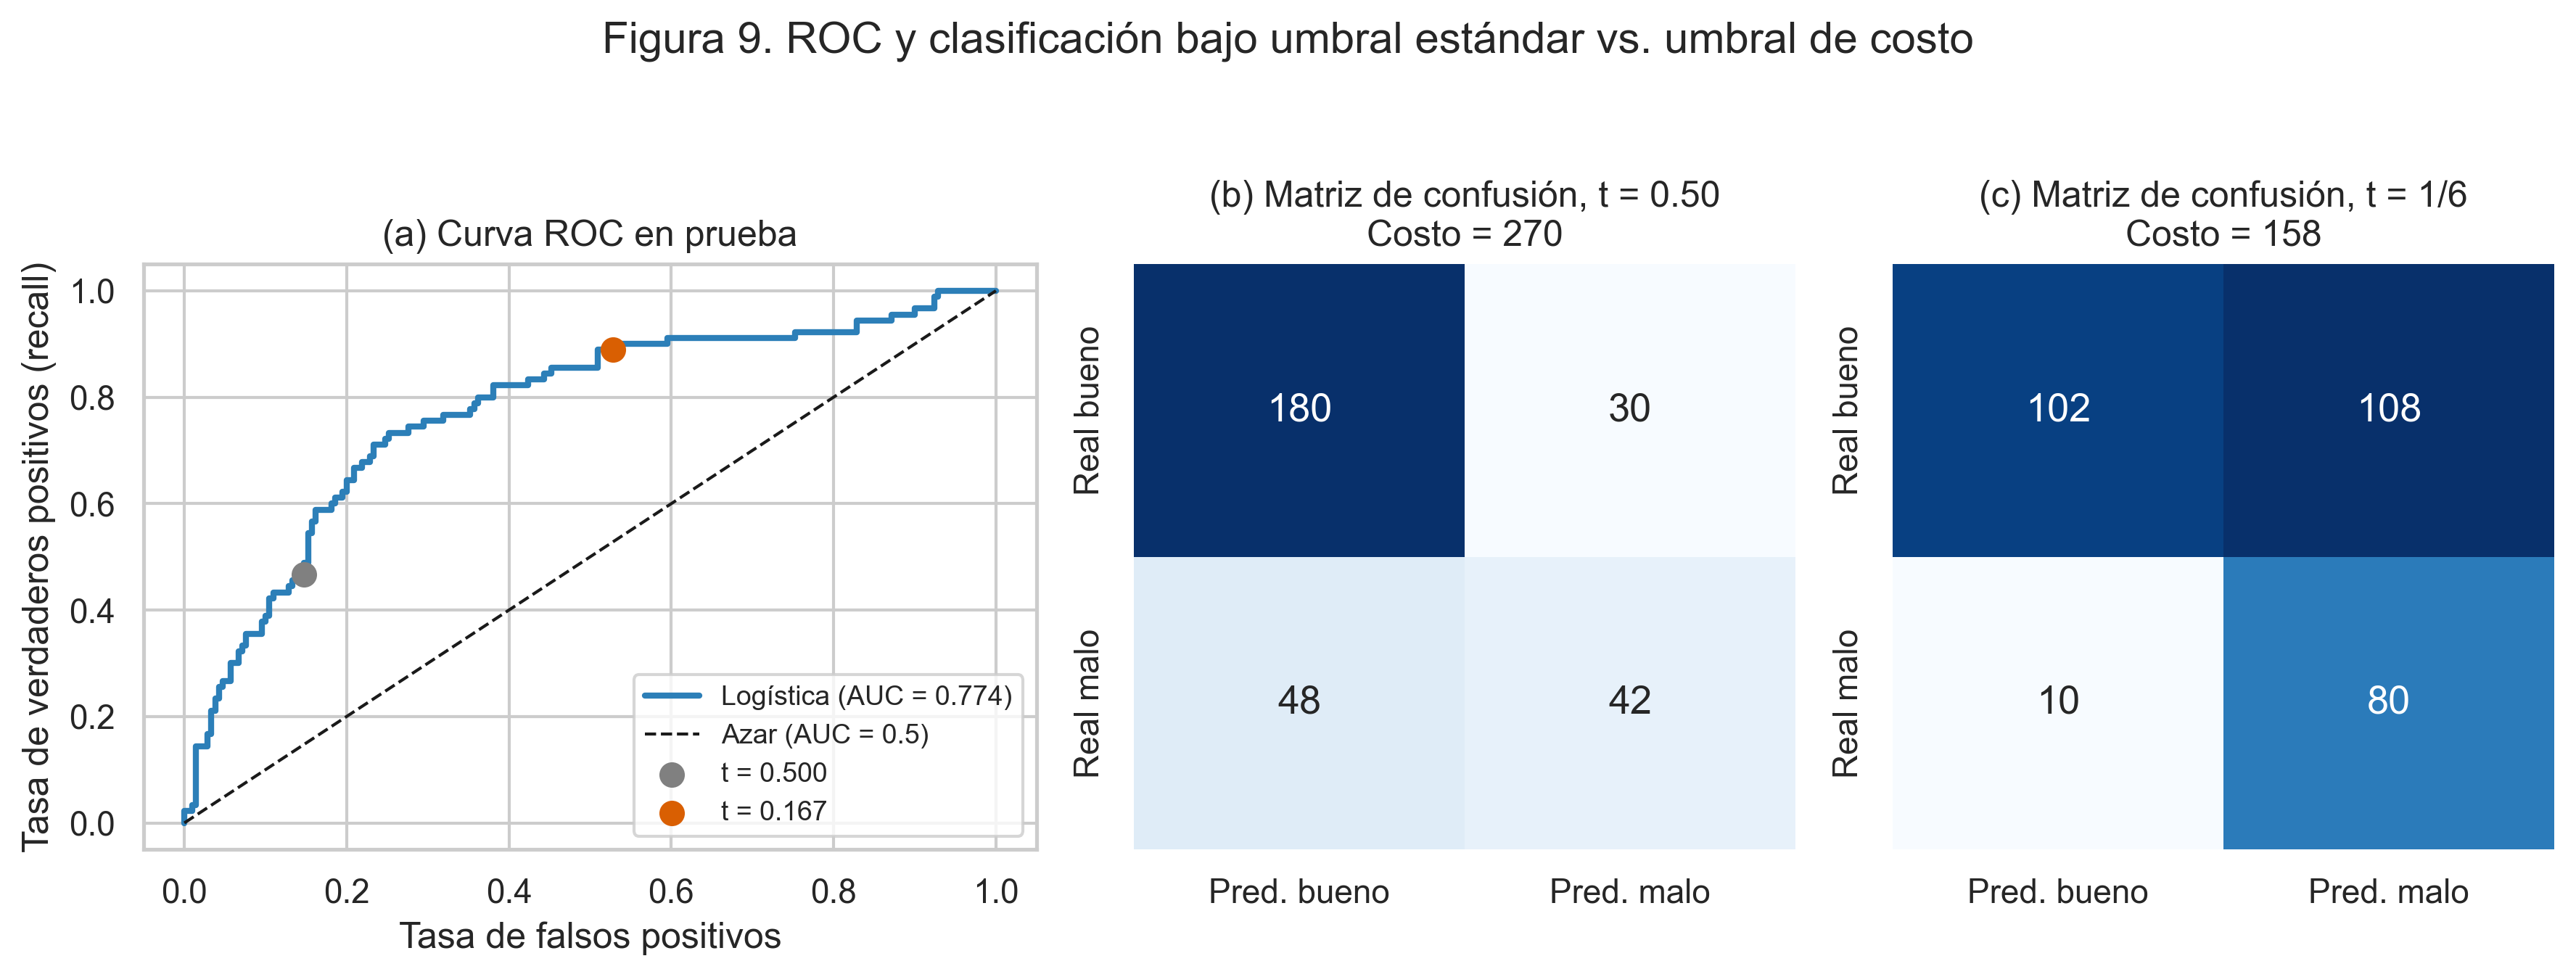
\includegraphics[
        width=\textwidth
    ]{
        figura_09_roc_y_matrices_confusion.png
    }

    \caption{
        Curva ROC y matrices de confusión del modelo logístico con el
        umbral estándar y el umbral derivado de la matriz de costos.
    }

    \label{fig:roc-matrices}
\end{figure}

La Figura~\ref{fig:roc-matrices} muestra que la curva ROC no cambia al
modificar el umbral: la capacidad de ordenamiento pertenece al modelo.
Lo que cambia es el punto de operación elegido sobre esa curva y, por
tanto, el equilibrio entre falsos positivos y falsos negativos.

\begin{hallazgo}
El umbral \(0.50\) ofrece mayor exactitud y especificidad, pero omite más
de la mitad de los malos créditos. Bajo la matriz de costos \(5:1\), el
umbral \(1/6\) reduce el costo total en aproximadamente \(41.5\,\%\) al
priorizar la detección del riesgo.
\end{hallazgo}

\subsection{Lectura operativa del modelo}

Los resultados permiten diferenciar tres propiedades del sistema:

\begin{enumerate}
    \item \textbf{Asociación.} Los odds ratios identifican variables que
    mantienen una relación condicional con la clase de riesgo.

    \item \textbf{Discriminación.} La AUC y el KS evalúan la capacidad
    para ordenar solicitantes desde menor hasta mayor riesgo.

    \item \textbf{Decisión.} El umbral transforma las probabilidades en
    una política de clasificación y determina el costo de los errores.
\end{enumerate}

Un modelo puede discriminar razonablemente y aun así producir una política
inadecuada si se utiliza un umbral incompatible con los costos del
negocio. De forma similar, un umbral conservador puede reducir pérdidas
por falsos negativos, pero también aumentar rechazos innecesarios.

La matriz \(5:1\) procede de la documentación del dataset y permite
desarrollar el ejercicio de decisión. No representa una estimación
económica completa de una institución. En una aplicación real, el costo
de un falso negativo debería incorporar exposición al incumplimiento,
pérdida dado incumplimiento, recuperación y costos de cobranza. El costo
de un falso positivo debería considerar margen financiero perdido,
costos de adquisición y valor futuro del cliente.

La elección final también requeriría:

\begin{itemize}
    \item evaluar la calibración de las probabilidades;

    \item validar temporalmente el modelo;

    \item comprobar la estabilidad de las variables y categorías;

    \item analizar equidad y posibles efectos adversos;

    \item establecer una zona de revisión manual para probabilidades
    cercanas al punto de corte.
\end{itemize}

Por tanto, el modelo debe considerarse una herramienta de apoyo para
priorizar y revisar solicitudes, no un mecanismo autónomo listo para
aprobar o rechazar créditos.

\subsection{Conclusión del modelamiento}

El modelo OLS mostró que la duración y la carga de la cuota explican una
parte importante de la estructura del monto otorgado, con un desempeño
estable en validación cruzada.

La regresión logística alcanzó una AUC de \(0.7740\) en prueba y una AUC
media de \(0.7685\) en validación cruzada. Esta consistencia indica una
capacidad discriminativa estable y sin evidencia importante de
sobreajuste bajo las particiones evaluadas.

Los factores condicionales más relevantes fueron el estado de la cuenta,
la duración, el historial crediticio, el nivel de ahorros, la vivienda y
la carga de la cuota. El monto mostró una asociación marginal con el
riesgo, pero perdió significancia al controlar simultáneamente por los
demás predictores.

Finalmente, la comparación de umbrales mostró que la política de decisión
no debe basarse exclusivamente en la exactitud. Bajo el costo asimétrico
\(5:1\), reducir el umbral a \(1/6\) aumenta sustancialmente la detección
de malos créditos y reduce el costo total, aunque a cambio de más falsos
positivos.


% 10.1 Modelo OLS auxiliar.
% 10.2 VIF y especificación.
% 10.3 Cuatro diagnósticos canónicos.
% 10.4 Test formal de supuestos.
% 10.5 Validación cruzada k-fold.
% 10.6 Regresión logística para mal riesgo.
% 10.7 Odds ratios e intervalos.
% 10.8 ROC--AUC, precision, recall y matrices de confusión.
% 10.9 Umbral 0,50 frente a umbral basado en costo 5:1.

\section{Análisis bayesiano}
\label{sec:bayes}

El análisis bayesiano complementa la inferencia frecuentista mediante una
representación probabilística de la incertidumbre sobre los parámetros.
Se desarrollaron dos ejercicios:

\begin{enumerate}
    \item un modelo Beta--Binomial conjugado para la proporción global de
    malos créditos;

    \item una regresión logística bayesiana estimada mediante
    Metropolis--Hastings para estudiar la distribución posterior del
    coeficiente de duración.
\end{enumerate}

El primer ejercicio permite obtener la distribución posterior de forma
analítica y evaluar la sensibilidad de los resultados frente a distintas
distribuciones previas. El segundo requiere simulación MCMC porque la
regresión logística no dispone de una posterior conjugada de forma
cerrada.

\subsection{Modelo Beta--Binomial para la tasa de mal crédito}
\label{subsec:beta-binomial}

En el enfoque frecuentista, la tasa de mal crédito se trató como un
parámetro fijo pero desconocido. A partir de:

\[
x=300,
\qquad
n=1000,
\]

se obtuvo la estimación:

\[
\widehat{p}
=
\frac{x}{n}
=
0.300.
\]

En el enfoque bayesiano, la incertidumbre sobre \(p\) se representa
mediante una distribución de probabilidad. Después de observar los datos,
la distribución previa se actualiza aplicando el teorema de Bayes:

\[
\pi(p\mid x)
\propto
L(x\mid p)\pi(p),
\]

donde:

\begin{itemize}
    \item \(\pi(p)\) es la distribución previa o \textit{prior};

    \item \(L(x\mid p)\) es la verosimilitud aportada por los datos;

    \item \(\pi(p\mid x)\) es la distribución posterior.
\end{itemize}

El resultado no es únicamente una estimación puntual, sino una
distribución completa que describe qué valores de \(p\) son más
compatibles con el prior y la información observada.

\subsubsection{Verosimilitud binomial}

Sea \(X\) el número de malos créditos observados entre \(n\) registros.
El modelo de muestreo es:

\[
X\mid p
\sim
\operatorname{Binomial}(n,p).
\]

La función de probabilidad es:

\[
\Pr(X=x\mid p)
=
\binom{n}{x}
p^x(1-p)^{n-x}.
\]

Para la inferencia sobre \(p\), los términos que no dependen del
parámetro pueden omitirse. La verosimilitud queda expresada como:

\[
L(p\mid x)
\propto
p^x(1-p)^{n-x}.
\]

En el problema analizado:

\[
L(p\mid x)
\propto
p^{300}(1-p)^{700}.
\]

\subsubsection{Distribución previa Beta}

Se asigna a la tasa una distribución previa:

\[
p
\sim
\operatorname{Beta}(\alpha,\beta).
\]

Su densidad es:

\[
\pi(p)
=
\frac{
    1
}{
    B(\alpha,\beta)
}
p^{\alpha-1}
(1-p)^{\beta-1},
\qquad
0<p<1,
\]

donde \(B(\alpha,\beta)\) es la función Beta.

Omitiendo la constante de normalización:

\[
\pi(p)
\propto
p^{\alpha-1}
(1-p)^{\beta-1}.
\]

La media previa es:

\[
\operatorname{E}[p]
=
\frac{\alpha}{\alpha+\beta}.
\]

Los parámetros \(\alpha\) y \(\beta\) controlan tanto la localización como
la concentración de la información previa.

\subsubsection{Posterior conjugada}

Al combinar el prior y la verosimilitud:

\[
\begin{aligned}
\pi(p\mid x)
&\propto
p^x(1-p)^{n-x}
p^{\alpha-1}(1-p)^{\beta-1}\\
&\propto
p^{\alpha+x-1}
(1-p)^{\beta+n-x-1}.
\end{aligned}
\]

Este núcleo corresponde nuevamente a una distribución Beta. Por tanto:

\[
p\mid X=x
\sim
\operatorname{Beta}
\left(
    \alpha+x,\,
    \beta+n-x
\right).
\]

La actualización puede interpretarse como la incorporación de \(x\)
malos créditos al primer parámetro y \(n-x\) buenos créditos al segundo:

\[
\alpha_{\mathrm{post}}
=
\alpha+x,
\]

\[
\beta_{\mathrm{post}}
=
\beta+n-x.
\]

Esta propiedad se denomina conjugación. Permite obtener la posterior
analíticamente, sin recurrir a métodos de simulación.

\subsection{Resúmenes de la distribución posterior}

Para cada prior se calcularon tres resúmenes: la media posterior, la
estimación MAP y el intervalo creíble del \(95\,\%\).

\subsubsection{Media posterior}

La media posterior es:

\[
\operatorname{E}[p\mid x]
=
\frac{
    \alpha+x
}{
    \alpha+\beta+n
}.
\]

Esta cantidad representa el valor esperado de la tasa después de combinar
la información previa con los datos.

\subsubsection{Estimación MAP}

La estimación de máxima densidad posterior es:

\[
\widehat{p}_{\mathrm{MAP}}
=
\frac{
    \alpha+x-1
}{
    \alpha+\beta+n-2
},
\]

siempre que los dos parámetros posteriores sean mayores que uno.

El MAP identifica el valor de \(p\) donde la densidad posterior alcanza
su máximo.

\subsubsection{Intervalo creíble}

El intervalo creíble central del \(95\,\%\) se obtiene con los cuantiles
\(0.025\) y \(0.975\) de la posterior:

\[
\Pr
\left(
    p_{\mathrm{inf}}
    \leq
    p
    \leq
    p_{\mathrm{sup}}
    \mid x
\right)
=
0.95.
\]

A diferencia de un intervalo de confianza frecuentista, este intervalo
permite una interpretación probabilística directa: condicionados al
prior y a los datos observados, la probabilidad posterior de que \(p\)
se encuentre entre ambos límites es del \(95\,\%\).

\subsection{Distribuciones previas evaluadas}

Se compararon tres priors con distintos niveles de información.

\subsubsection{Prior uniforme}

El primer modelo utiliza:

\[
p
\sim
\operatorname{Beta}(1,1).
\]

Esta distribución es uniforme en el intervalo \([0,1]\):

\[
\pi(p)=1.
\]

Antes de observar los datos, asigna la misma densidad a cualquier valor
posible de la tasa. Se utiliza como una especificación inicial poco
informativa.

La posterior resultante es:

\[
p\mid x
\sim
\operatorname{Beta}(301,701).
\]

\subsubsection{Prior de Jeffreys}

El segundo modelo utiliza:

\[
p
\sim
\operatorname{Beta}(0.5,0.5).
\]

El prior de Jeffreys es una alternativa no informativa construida a
partir de la información de Fisher del modelo binomial. Su densidad
asigna mayor peso a los extremos del intervalo que el prior uniforme.

La posterior es:

\[
p\mid x
\sim
\operatorname{Beta}(300.5,700.5).
\]

Su inclusión permite comprobar si una definición no informativa diferente
produce cambios apreciables en la inferencia.

\subsubsection{Prior informativo débil}

El tercer modelo utiliza:

\[
p
\sim
\operatorname{Beta}(6,18).
\]

Su media previa es:

\[
\operatorname{E}[p]
=
\frac{6}{6+18}
=
0.25.
\]

La concentración total es:

\[
\alpha+\beta
=
24.
\]

Este prior representa una expectativa inicial de que la tasa se encuentre
alrededor del \(25\,\%\), pero con una concentración pequeña frente a las
\(1000\) observaciones disponibles. Por ello, se considera informativo
débil.

La posterior resultante es:

\[
p\mid x
\sim
\operatorname{Beta}(306,718).
\]

El propósito de este prior no es imponer una tasa de \(25\,\%\), sino
evaluar cuánto se desplaza la inferencia cuando se incorpora una
expectativa previa moderadamente distinta de la tasa observada.

\subsection{Resultados posteriores}

La Tabla~\ref{tab:resultados-beta-binomial} presenta los resultados para
los tres priors.

\begin{table}[H]
    \centering
    \caption{Resultados del modelo Beta--Binomial bajo diferentes
    distribuciones previas.}
    \label{tab:resultados-beta-binomial}

    \small
    \begin{tabularx}{0.98\textwidth}{
        @{}
        >{\raggedright\arraybackslash}p{3.4cm}
        >{\centering\arraybackslash}p{2.5cm}
        >{\centering\arraybackslash}p{1.6cm}
        >{\centering\arraybackslash}p{1.8cm}
        X
        @{}
    }
        \toprule
        Prior
        & Posterior
        & MAP
        & Media
        & Intervalo creíble del \(95\,\%\) \\
        \midrule

        \(\operatorname{Beta}(1,1)\), uniforme
        & \(\operatorname{Beta}(301,701)\)
        & \num{0.3000}
        & \num{0.3004}
        & \([0.2724,\;0.3291]\) \\

        \(\operatorname{Beta}(0.5,0.5)\), Jeffreys
        & \(\operatorname{Beta}(300.5,700.5)\)
        & \num{0.2998}
        & \num{0.3002}
        & \([0.2722,\;0.3289]\) \\

        \(\operatorname{Beta}(6,18)\), informativo débil
        & \(\operatorname{Beta}(306,718)\)
        & \num{0.2984}
        & \num{0.2988}
        & \([0.2712,\;0.3272]\) \\

        \bottomrule
    \end{tabularx}
\end{table}

Los tres modelos producen resultados muy próximos. Las estimaciones MAP
se encuentran entre:

\[
0.2984
\quad\text{y}\quad
0.3000,
\]

mientras que las medias posteriores se sitúan entre:

\[
0.2988
\quad\text{y}\quad
0.3004.
\]

El prior uniforme produce un MAP de \(0.3000\), coincidente con la
estimación frecuentista. El prior de Jeffreys genera un resultado casi
idéntico.

El prior \(\operatorname{Beta}(6,18)\) desplaza ligeramente la posterior
hacia su media previa de \(0.25\). Sin embargo, la media posterior solo
disminuye hasta \(0.2988\), lo que muestra que la influencia del prior es
reducida frente al tamaño de la muestra.

\subsection{Sensibilidad al prior}

La Figura~\ref{fig:beta-binomial} compara las distribuciones previas y
posteriores.

\begin{figure}[H]
    \centering

    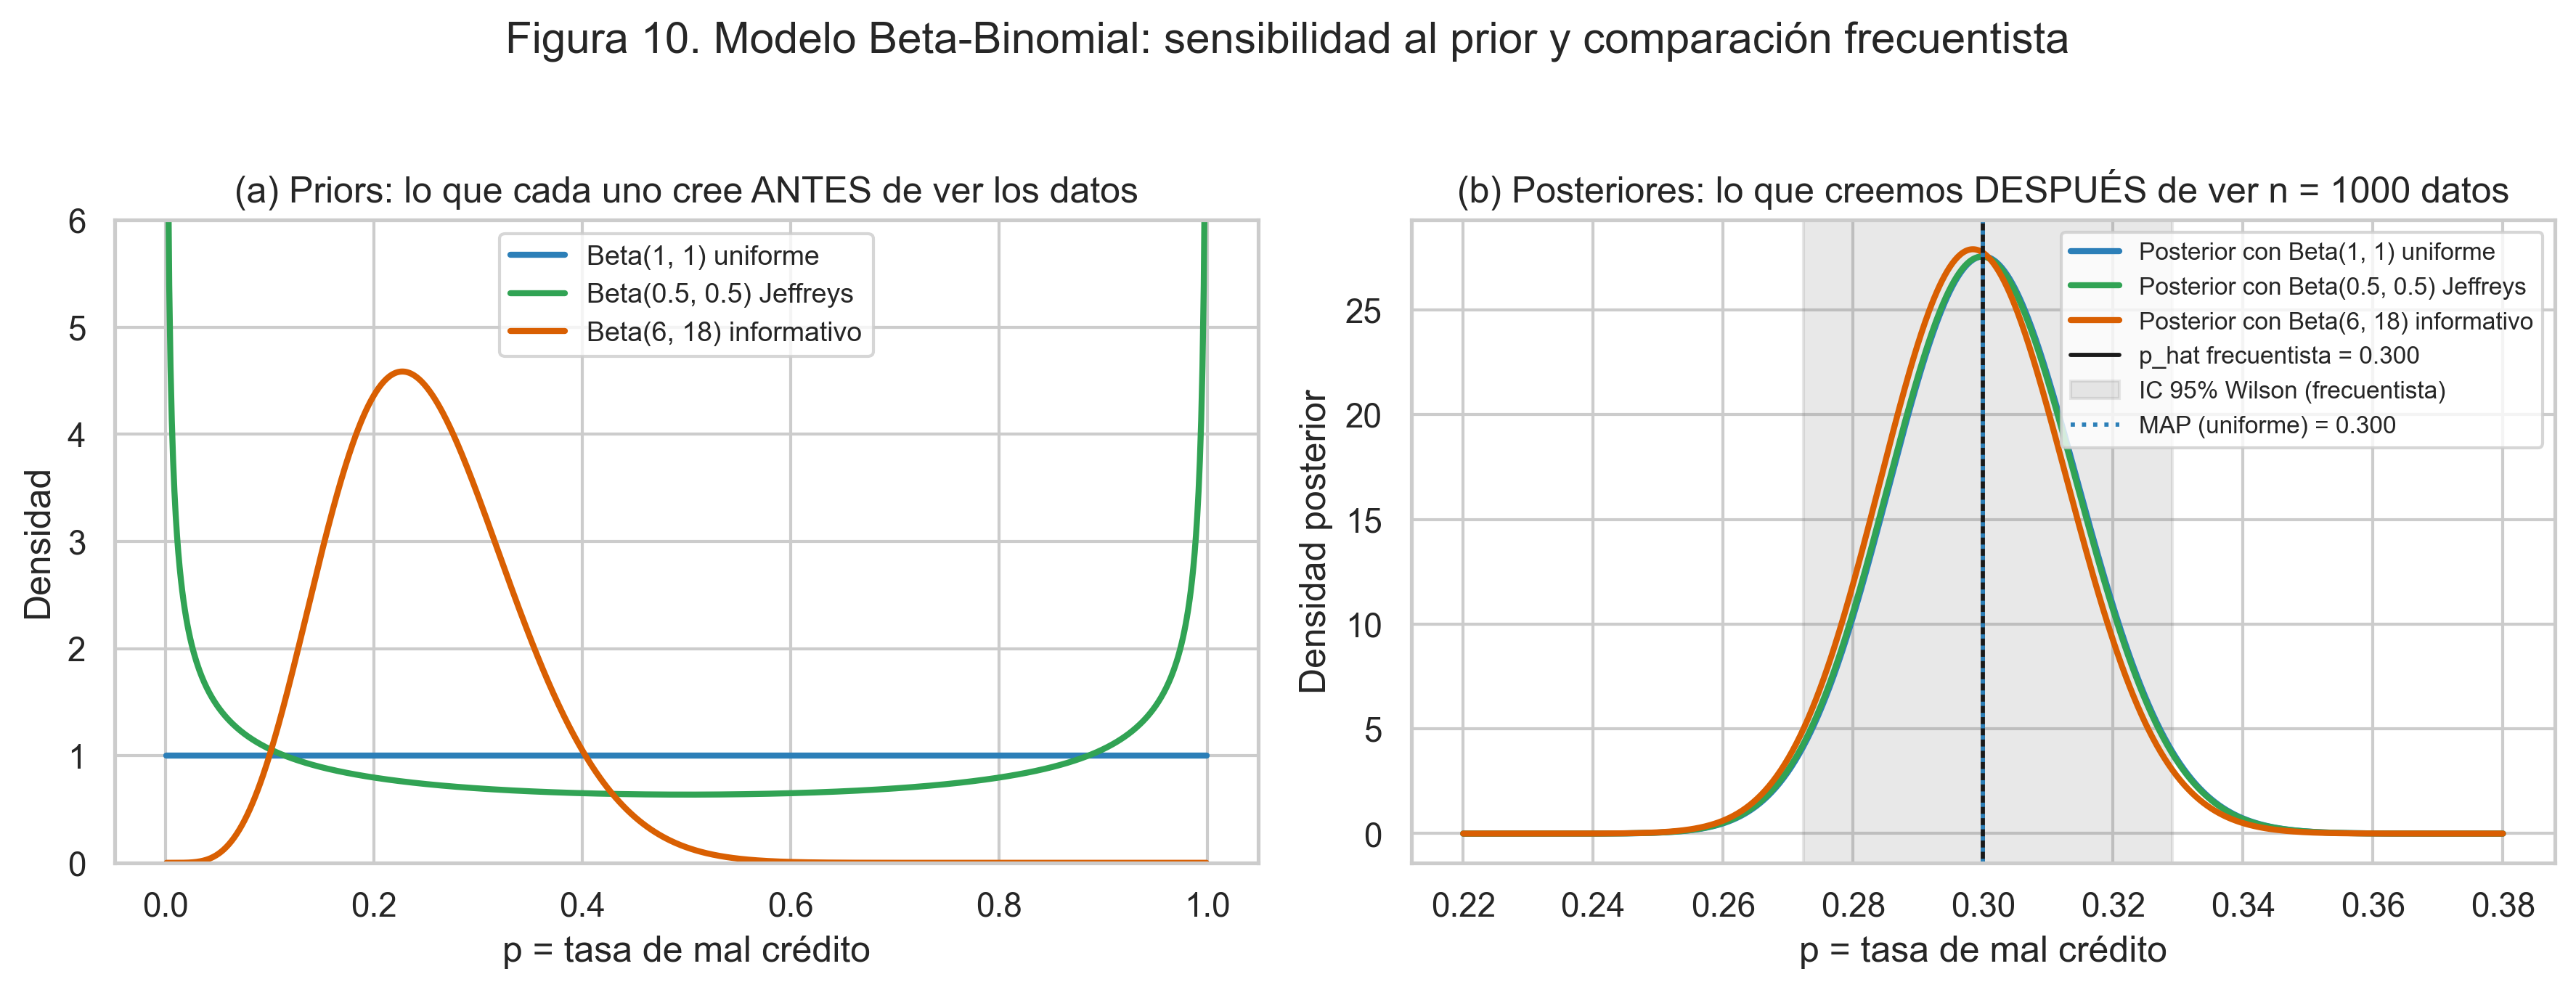
\includegraphics[
        width=\textwidth
    ]{
        figura_10_modelo_beta_binomial.png
    }

    \caption{
        Sensibilidad del modelo Beta--Binomial a la elección del prior.
        El panel izquierdo muestra las tres distribuciones previas. El
        panel derecho presenta las posteriores, la estimación
        frecuentista y el intervalo de Wilson del \(95\,\%\).
    }

    \label{fig:beta-binomial}
\end{figure}

En el panel izquierdo, los priors presentan formas claramente diferentes.
El uniforme asigna densidad constante, Jeffreys concentra más densidad
cerca de cero y uno, y el prior informativo concentra su masa alrededor
de valores próximos a \(0.25\).

Después de observar los \(1000\) registros, las tres posteriores se
superponen casi completamente. La evidencia contenida en los datos domina
las diferencias entre las distribuciones previas.

La amplitud de los intervalos creíbles también es muy similar. Entre el
límite inferior más bajo y el más alto existe una diferencia de apenas:

\[
0.2724-0.2712
=
0.0012,
\]

equivalente a \(0.12\) puntos porcentuales. Entre los límites superiores,
la diferencia máxima es:

\[
0.3291-0.3272
=
0.0019,
\]

equivalente a \(0.19\) puntos porcentuales.

Estas variaciones no modifican la conclusión sustantiva: la tasa de mal
crédito se concentra alrededor del \(30\,\%\).

\begin{hallazgo}
La inferencia sobre la tasa de mal crédito es robusta frente a los tres
priors considerados. Con \(n=1000\), los datos dominan la actualización
y mantienen la media posterior próxima a \(0.30\).
\end{hallazgo}

\subsection{Comparación con la inferencia frecuentista}

En la Sección~\ref{sec:incertidumbre}, el intervalo de Wilson fue:

\[
\operatorname{IC}_{95\,\%,\,\mathrm{Wilson}}
=
[0.2724,\;0.3291].
\]

Con el prior uniforme, el intervalo creíble fue:

\[
\operatorname{ICr}_{95\,\%,\,\mathrm{Beta}(1,1)}
=
[0.2724,\;0.3291].
\]

Los límites coinciden numéricamente al nivel de redondeo utilizado. Esta
coincidencia no significa que ambos intervalos sean conceptualmente
iguales.

El intervalo de Wilson se interpreta como una propiedad de un
procedimiento repetido: en un conjunto hipotético de muestras comparables,
aproximadamente el \(95\,\%\) de los intervalos construidos mediante
Wilson contendría el verdadero valor de \(p\).

El intervalo creíble responde a una afirmación distinta:

\[
\Pr
\left(
    0.2724
    \leq
    p
    \leq
    0.3291
    \mid x
\right)
=
0.95,
\]

condicionada al modelo binomial, al prior uniforme y a los datos
observados.

La similitud numérica se explica por el tamaño de la muestra y por el uso
de un prior débil. En estas condiciones, tanto la aproximación
frecuentista como la posterior se concentran cerca de la proporción
muestral.

\begin{table}[H]
    \centering
    \caption{Comparación entre la inferencia frecuentista y bayesiana
    para la tasa de mal crédito.}
    \label{tab:comparacion-frecuentista-bayes}

    \begin{tabularx}{0.94\textwidth}{
        @{}
        >{\raggedright\arraybackslash}p{3.5cm}
        >{\centering\arraybackslash}p{2.2cm}
        >{\centering\arraybackslash}p{3.0cm}
        X
        @{}
    }
        \toprule
        Enfoque
        & Estimación
        & Intervalo del \(95\,\%\)
        & Interpretación \\
        \midrule

        Frecuentista: Wilson
        & \(\widehat{p}=0.3000\)
        & \([0.2724,\;0.3291]\)
        & Cobertura del procedimiento bajo muestreo repetido. \\

        Bayesiano:
        \(\operatorname{Beta}(1,1)\)
        & MAP \(=0.3000\)
        & \([0.2724,\;0.3291]\)
        & Probabilidad posterior condicionada al prior y los datos. \\

        \bottomrule
    \end{tabularx}
\end{table}

Ambos enfoques conducen a la misma conclusión aplicada: la tasa de mal
crédito del conjunto analizado se estima cerca del \(30\,\%\), con una
incertidumbre aproximada de tres puntos porcentuales a cada lado.

\subsection{Supuestos y alcance del modelo}

El modelo Beta--Binomial supone que, condicionado a \(p\), los registros
pueden representarse como ensayos Bernoulli comparables e independientes.
También supone una única tasa común para toda la muestra.

Esta simplificación ignora posibles diferencias entre propósitos,
duraciones, perfiles financieros o periodos de originación. El modelo
describe la tasa agregada de la cartera, pero no sustituye la regresión
logística utilizada para estimar probabilidades condicionales.

La posterior tampoco corrige problemas de representatividad de la
muestra. Una distribución posterior estrecha puede reflejar alta precisión
condicionada al dataset y, al mismo tiempo, coexistir con una validez
externa limitada.

Por tanto, el intervalo creíble cuantifica la incertidumbre estadística
sobre la tasa dentro del modelo asumido. No garantiza que la misma tasa
sea aplicable a otra institución, país o periodo.

% ============================================================
% En el siguiente bloque se incorporarán:
% - Regresión logística bayesiana
% - Prior normal débilmente informativo
% - Metropolis--Hastings multivariante
% - Diagnósticos de la cadena
% - Posterior del coeficiente de duración
% ============================================================

% Contenido previsto:
% - Modelo Beta--Binomial.
% - Prior, verosimilitud y posterior conjugada.
% - Media posterior, MAP e intervalo creíble al 95 %.
% - Sensibilidad a por lo menos dos priors.
% - Comparación con el IC de Wilson.
% - Metropolis--Hastings para un coeficiente logístico.
% - Diagnóstico de cadena e interpretación posterior.

\section{Interpretación integrada}
\label{sec:interpretacion-integrada}

La pregunta central del trabajo fue:

\begin{quote}
    \itshape
    ¿Qué factores explican la probabilidad de que un solicitante sea
    clasificado como mal riesgo crediticio?
\end{quote}

La evidencia obtenida muestra que el riesgo crediticio no se concentra
en una única característica. La clasificación depende de una combinación
entre las condiciones del préstamo, la liquidez disponible, los
antecedentes financieros y algunos indicadores de estabilidad económica.

El término ``explican'' se utiliza en un sentido estadístico y
predictivo. Los resultados permiten identificar variables asociadas con
cambios en la probabilidad estimada de mal crédito, pero no demuestran
que esas variables causen directamente el resultado observado.

\subsection{Respuesta a la pregunta central}

Dentro de las variables numéricas, la duración del préstamo constituye
el factor con la asociación más consistente. Los créditos clasificados
como malos presentan plazos mayores en el análisis descriptivo, una
diferencia estandarizada cercana a moderada en la comparación
frecuentista y un coeficiente positivo en la regresión logística.

En el modelo multivariable, cada mes adicional de duración se asocia con
un incremento aproximado del \(3.9\,\%\) en las \textit{odds} de mal
crédito, manteniendo constantes los demás predictores. El análisis
bayesiano confirmó este resultado:

\[
\operatorname{E}
\left[
    \beta_{\mathrm{dur}}
    \mid
    \mathrm{datos}
\right]
=
0.04084,
\]

\[
\operatorname{ICr}_{95\,\%}
=
[0.01902,\;0.06275],
\]

y:

\[
\Pr
\left(
    \beta_{\mathrm{dur}}>0
    \mid
    \mathrm{datos}
\right)
\approx
1.
\]

Por tanto, la duración es el principal factor numérico asociado con un
mayor riesgo dentro de la especificación utilizada.

La carga de la cuota también mantiene una asociación condicional
relevante. Una unidad adicional en la escala ordinal de
\variable{tasa_cuota} se relaciona con un aumento aproximado del
\(22.8\,\%\) en las \textit{odds} de mal crédito:

\[
\mathrm{OR}=1.2283.
\]

Este resultado es coherente con la interpretación financiera de que una
mayor proporción de recursos comprometida en el pago puede reducir el
margen disponible frente a gastos inesperados. No obstante, la variable
representa niveles ordinales y no porcentajes exactos del ingreso.

Entre las variables categóricas, el estado de la cuenta corriente, el
nivel de ahorros, algunas categorías del historial crediticio, la
antigüedad laboral y el tipo de vivienda aportan información adicional.
En términos generales, los perfiles con mejores señales de liquidez o
estabilidad presentan menores \textit{odds} de mal crédito respecto de
sus categorías de referencia.

La interpretación de estas categorías requiere cautela. Algunos códigos
históricos combinan situaciones diferentes y ciertas asociaciones pueden
parecer contraintuitivas debido a la categoría utilizada como referencia.
En consecuencia, no deben convertirse directamente en reglas generales
de aprobación o rechazo.

\subsection{Diferencia entre asociación marginal y condicional}

Uno de los resultados más importantes del análisis es la diferencia entre
una asociación observada por separado y una asociación que permanece al
controlar por otras variables.

El monto del crédito mostró inicialmente:

\begin{itemize}
    \item valores medios y medianos superiores entre los malos créditos;

    \item una diferencia estadísticamente significativa mediante
    Mann--Whitney;

    \item una asociación positiva, aunque pequeña, con la clase de
    riesgo.
\end{itemize}

Sin embargo, dentro de la regresión logística:

\[
\mathrm{OR}_{\log(\mathrm{monto})}
=
1.0658,
\]

con:

\[
p=0.7238.
\]

El intervalo del \(95\,\%\) contiene el valor uno. Por tanto, no existe
evidencia suficiente de una asociación independiente del monto después
de considerar duración, estado de cuenta, historial, ahorros, carga de
la cuota y vivienda.

Este cambio es coherente con la relación observada entre monto y
duración:

\[
\rho_{\mathrm{Spearman}}
\approx
0.62.
\]

Los créditos de mayor monto tienden a concederse por plazos más largos.
En consecuencia, parte de la asociación marginal del monto con el riesgo
parece estar capturada por la duración y por otras condiciones
financieras.

La edad presenta un comportamiento parecido. Los malos créditos
corresponden descriptivamente a solicitantes algo más jóvenes, pero la
edad no conserva evidencia estadística dentro del modelo logístico:

\[
\mathrm{OR}_{\mathrm{edad}}
=
0.9972,
\qquad
p=0.7798.
\]

Por tanto, ni el monto ni la edad deben considerarse factores
condicionales principales en la especificación final.

\subsection{Propósito del préstamo como factor de segmentación}

La prueba chi-cuadrado identificó una asociación entre el propósito y la
clase de riesgo:

\[
\chi^2(9)
=
33.356,
\qquad
p=0.00012.
\]

La magnitud estimada mediante V de Cramér fue:

\[
V=0.183.
\]

Esto indica una asociación global estadísticamente significativa, pero
pequeña. Algunos propósitos presentan tasas observadas superiores al
promedio, mientras que otros muestran tasas menores.

Sin embargo, el propósito debe entenderse principalmente como una
variable de segmentación. Las tasas de algunas categorías se basan en
pocos registros y pueden ser inestables. Además, la prueba global no
controla por duración, monto, liquidez ni situación financiera.

Por ello, el propósito aporta contexto sobre el tipo de operación, pero
no constituye por sí solo una base suficiente para determinar el riesgo
individual de un solicitante.

\subsection{Síntesis de la evidencia por factor}

La Tabla~\ref{tab:evidencia-integrada-factores} resume la relación entre
los principales factores y el riesgo.

\begin{table}[H]
    \centering
    \caption{Síntesis integrada de los factores asociados con el riesgo
    crediticio.}
    \label{tab:evidencia-integrada-factores}

    \small
    \begin{tabularx}{\textwidth}{
        @{}
        >{\raggedright\arraybackslash}p{2.7cm}
        >{\raggedright\arraybackslash}p{4.1cm}
        >{\raggedright\arraybackslash}p{4.0cm}
        X
        @{}
    }
        \toprule
        Factor
        & Evidencia marginal
        & Evidencia condicional
        & Interpretación integrada \\
        \midrule

        Duración
        & Los malos créditos tienen plazos mayores; \(d=0.480\).
        & \(\mathrm{OR}=1.0390\) por mes; posterior completamente
          concentrada en valores positivos.
        & Factor numérico más consistente del análisis. \\

        Tasa de la cuota
        & Mayor presencia de niveles altos entre los malos créditos.
        & \(\mathrm{OR}=1.2283\), con intervalo por encima de uno.
        & Una mayor carga financiera se asocia con mayor riesgo. \\

        Monto
        & Diferencia significativa entre clases; efecto pequeño.
        & \(\mathrm{OR}=1.0658\), \(p=0.7238\).
        & Su asociación marginal no permanece después del control
          multivariable. \\

        Estado de cuenta
        & Diferencias visibles entre perfiles de liquidez.
        & Varias categorías presentan \(\mathrm{OR}<1\) frente al saldo
          negativo.
        & La liquidez corriente aporta una señal condicional importante. \\

        Ahorros
        & Los perfiles con mayor ahorro muestran menor riesgo observado.
        & \texttt{A64}: \(\mathrm{OR}=0.1617\) frente a menos de
          \(100\) DM.
        & Una mayor capacidad de ahorro se asocia con menor riesgo. \\

        Historial crediticio
        & Las tasas cambian entre categorías.
        & Algunas categorías presentan asociaciones significativas
          respecto de \texttt{A30}.
        & Aporta información, pero depende fuertemente de la referencia
          y de la codificación histórica. \\

        Vivienda
        & La distribución de las clases varía según el régimen de
          vivienda.
        & Vivienda propia:
          \(\mathrm{OR}=0.5868\) frente al alquiler.
        & La estabilidad residencial se asocia con menores
          \textit{odds}. \\

        Propósito
        & Asociación global significativa, \(V=0.183\).
        & No se utilizó como predictor en la especificación logística
          final.
        & Útil para segmentación, con capacidad individual limitada. \\

        Edad
        & Los malos créditos son ligeramente más jóvenes.
        & \(\mathrm{OR}=0.9972\), \(p=0.7798\).
        & La diferencia marginal no persiste en el modelo conjunto. \\

        \bottomrule
    \end{tabularx}
\end{table}

\subsection{Respuesta a las preguntas secundarias}

Las preguntas específicas del trabajo pueden responderse de manera
integrada.

\subsubsection{¿Cuál es la proporción global de malos créditos?}

La proporción observada fue:

\[
\widehat{p}
=
0.300.
\]

El intervalo de Wilson del \(95\,\%\) fue:

\[
[0.2724,\;0.3291],
\]

mientras que el intervalo bootstrap fue:

\[
[0.2720,\;0.3290].
\]

El modelo Beta--Binomial produjo intervalos creíbles prácticamente
idénticos bajo los tres priors evaluados. La tasa se estima, por tanto,
cerca del \(30\,\%\), con una incertidumbre aproximada de tres puntos
porcentuales a cada lado.

\subsubsection{¿La tasa difiere según el propósito?}

Sí. La prueba chi-cuadrado rechazó la hipótesis de independencia entre
propósito y clase de riesgo. Sin embargo, la V de Cramér de \(0.183\)
indica que la magnitud de la asociación es pequeña.

El propósito permite reconocer segmentos con tasas diferentes, pero no
explica por sí solo la clasificación individual.

\subsubsection{¿La duración y el monto difieren entre las clases?}

Ambas variables presentan diferencias marginales.

Los malos créditos tienen una duración media aproximadamente
\(5.65\) meses mayor, con un tamaño de efecto:

\[
d=0.480.
\]

El monto también tiende a ser mayor, pero su tamaño de efecto es pequeño:

\[
r_{\mathrm{rb}}
=
0.110.
\]

La diferencia esencial aparece en el análisis multivariable: la duración
mantiene su asociación, mientras que el monto pierde significancia.

\subsubsection{¿Qué variables están asociadas con mayor riesgo?}

La evidencia conjunta identifica como señales principales:

\begin{itemize}
    \item mayor duración del crédito;

    \item mayor nivel de carga de la cuota;

    \item estado de cuenta menos favorable, especialmente la categoría
    de saldo negativo utilizada como referencia;

    \item menores niveles de ahorro;

    \item determinados perfiles del historial crediticio;

    \item menor estabilidad residencial frente a la vivienda propia.
\end{itemize}

La interpretación debe realizarse sobre el perfil completo. Ninguna
variable ofrece una separación perfecta entre buenos y malos créditos.

\subsubsection{¿Cómo cambia la clasificación al modificar el umbral?}

Con el umbral convencional:

\[
t=0.50,
\]

el modelo obtiene una exactitud de \(74.0\,\%\), pero identifica solo el
\(46.7\,\%\) de los malos créditos.

Bajo la relación de costos \(5:1\), el umbral teórico es:

\[
t^{*}
=
\frac{1}{6}
\approx
0.1667.
\]

Al aplicarlo, el recall aumenta a:

\[
88.9\,\%,
\]

y los falsos negativos disminuyen de \(48\) a \(10\). A cambio, los
falsos positivos aumentan y la exactitud disminuye al \(60.7\,\%\).

El costo total se reduce de:

\[
270
\quad\text{a}\quad
158,
\]

lo que representa una disminución aproximada del:

\[
41.5\,\%.
\]

La modificación del umbral no mejora la capacidad discriminativa del
modelo. Cambia la política de decisión y el equilibrio entre los dos
tipos de error.

\subsection{Coherencia entre los enfoques estadísticos}

Los resultados frecuentistas y bayesianos presentan una alta
consistencia.

Para la tasa global de mal crédito:

\[
\widehat{p}_{\mathrm{frecuentista}}
=
0.3000,
\]

mientras que, con el prior uniforme:

\[
\widehat{p}_{\mathrm{MAP}}
=
0.3000.
\]

El intervalo de Wilson y el intervalo creíble bajo
\(\operatorname{Beta}(1,1)\) coinciden numéricamente al nivel de redondeo:

\[
[0.2724,\;0.3291].
\]

Para la duración, el estimador frecuentista fue:

\[
\widehat{\beta}_{\mathrm{dur,MLE}}
=
0.03825,
\]

y la media posterior:

\[
\operatorname{E}
\left[
    \beta_{\mathrm{dur}}
    \mid
    \mathrm{datos}
\right]
=
0.04084.
\]

Las diferencias son pequeñas. Esta concordancia es esperable debido al
tamaño de la muestra y al uso de distribuciones previas débiles.

La similitud numérica no elimina la diferencia conceptual. La inferencia
frecuentista describe propiedades del procedimiento de estimación bajo
muestreo repetido. La inferencia bayesiana expresa incertidumbre
posterior condicionada al prior y a los datos observados.

\subsection{Predicción y utilidad operativa}

La regresión logística alcanzó:

\[
\operatorname{AUC}_{\mathrm{test}}
=
0.7740,
\]

y una media de validación cruzada de:

\[
\overline{\operatorname{AUC}}_{\mathrm{CV}}
=
0.7685
\pm
0.0221.
\]

La proximidad entre ambos resultados indica una capacidad discriminativa
estable dentro del esquema de evaluación utilizado.

Sin embargo, una AUC cercana a \(0.77\) no implica una clasificación
perfecta ni determina automáticamente una política crediticia adecuada.
El modelo ordena razonablemente los perfiles, pero existe un solapamiento
considerable entre las clases.

La utilidad operativa depende de tres niveles diferentes:

\begin{enumerate}
    \item \textbf{Estimación del riesgo:} producción de una probabilidad
    individual de mal crédito;

    \item \textbf{Discriminación:} capacidad de ordenar correctamente
    casos de mayor y menor riesgo;

    \item \textbf{Decisión:} elección de un umbral compatible con los
    costos y objetivos de la institución.
\end{enumerate}

Un modelo puede mostrar una discriminación estable y, al mismo tiempo,
producir decisiones costosas cuando se utiliza un umbral inadecuado.

\subsection{Implicancias para una política crediticia}

Los resultados sugieren que las operaciones de larga duración y elevada
carga de cuota requieren una revisión más cuidadosa. Esto no implica que
deban rechazarse automáticamente. Una política de gestión podría
considerar:

\begin{itemize}
    \item reducir el plazo cuando la capacidad de pago sea limitada;

    \item solicitar garantías adicionales en operaciones de mayor riesgo;

    \item ajustar el monto o la estructura de cuotas;

    \item establecer una revisión manual para probabilidades cercanas al
    umbral;

    \item incorporar información financiera más reciente antes de la
    decisión final.
\end{itemize}

El monto no debería utilizarse aisladamente como argumento de riesgo. Su
asociación marginal desaparece después de considerar la duración y otras
características.

Del mismo modo, categorías personales o históricas no deben convertirse
automáticamente en reglas de exclusión. Su utilización debe someterse a
criterios de pertinencia, equidad y regulación.

\subsection{Respuesta integrada final}

La probabilidad de mal riesgo crediticio se asocia principalmente con la
combinación de plazos prolongados, mayor carga de la cuota y señales menos
favorables de liquidez o estabilidad financiera.

La duración es el factor numérico más consistente: aparece en el análisis
exploratorio, la comparación frecuentista, la regresión logística y la
posterior bayesiana. El estado de cuenta, los ahorros, el historial
crediticio y la vivienda complementan esta señal.

El monto y la edad muestran diferencias marginales, pero no conservan
evidencia condicional dentro del modelo final. El propósito está asociado
globalmente con el riesgo, aunque su magnitud es pequeña y su utilidad
principal es la segmentación.

Finalmente, el desempeño del sistema no depende únicamente de la calidad
del modelo. La selección del umbral modifica sustancialmente los errores
y los costos. Bajo la matriz \(5:1\), el umbral \(1/6\) resulta más
coherente que \(0.50\), porque prioriza la detección de malos créditos y
reduce el costo total observado.

En consecuencia, el modelo debe entenderse como una herramienta de apoyo
a la decisión: combina información sobre el perfil y la operación,
produce una estimación de riesgo y permite adaptar la clasificación a los
costos del problema. No constituye una explicación causal ni un sistema
listo para despliegue sin validación externa, recalibración y revisión de
equidad.

% Contenido previsto:
% - Respuesta conjunta a las cinco preguntas del Grupo 5.
% - Diferencia entre asociación marginal y condicional.
% - Convergencia y divergencia entre resultados frecuentistas y bayesianos.
% - Implicancias operativas del umbral y los costos.

\section{Limitaciones y validez}
\label{sec:limitaciones}

% Contenido previsto:
% - Validez interna, externa y de constructo.
% - Antigüedad y contexto alemán del dataset.
% - Limitaciones de codificación y representatividad.
% - Ausencia de interpretación causal.
% - Riesgos éticos, sesgo y poblaciones vulnerables.
% - Necesidad de supervisión humana.

\section{Conclusiones}
\label{sec:conclusiones}

% Contenido previsto:
% - Síntesis de hallazgos.
% - Desempeño predictivo y límites.
% - Decisión de umbral.
% - Resultado bayesiano.
% - Recomendaciones técnicas y de uso responsable.

\section{Declaración de contribución individual}
\label{sec:contribuciones}

El trabajo fue desarrollado de manera colaborativa por los tres
integrantes del Grupo 5. Para organizar las responsabilidades, el
análisis se dividió en tres bloques temáticos coherentes: preparación y
exploración de los datos; inferencia frecuentista y regresión lineal; y
modelamiento predictivo e inferencia bayesiana.

La distribución porcentual representa la responsabilidad principal
asumida por cada integrante sobre el desarrollo, validación y
documentación de su bloque. Esta asignación no excluye la revisión
cruzada ni la participación conjunta en la interpretación de los
resultados.

La contribución total declarada es:

\[
40\,\% + 30\,\% + 30\,\% = 100\,\%.
\]

La Tabla~\ref{tab:contribuciones-individuales} resume la distribución
general de responsabilidades.

\begin{table}[H]
    \centering
    \caption{Distribución de las contribuciones individuales.}
    \label{tab:contribuciones-individuales}

    \small
    \begin{tabularx}{\textwidth}{
        @{}
        >{\raggedright\arraybackslash}p{3.1cm}
        >{\raggedright\arraybackslash}p{2.7cm}
        X
        @{}
    }
        \toprule
        Integrante
        & Bloque y participación
        & Responsabilidades principales \\
        \midrule

        Henry Sánchez Alvarado
        &
        \textbf{Bloque 1}

        Preparación, exploración e incertidumbre

        \textbf{40\,\%}
        &
        Organización general del flujo reproducible; documentación y
        carga del dataset; elaboración del diccionario de variables;
        validación, limpieza y recodificación de la respuesta; análisis
        exploratorio y estadística descriptiva; ajuste paramétrico del
        monto; desarrollo de las visualizaciones iniciales; estimación
        de intervalos de confianza mediante Wilson, bootstrap y
        distribución \(t\); integración de la estructura general del
        informe y revisión de la correspondencia entre notebook,
        resultados e informe.
        \\

        \addlinespace

        Armando Castro Chaupis
        &
        \textbf{Bloque 2}

        Inferencia frecuentista y regresión lineal

        \textbf{30\,\%}
        &
        Formulación y evaluación de las hipótesis frecuentistas;
        aplicación de la prueba chi-cuadrado y cálculo de la V de
        Cramér; comparación de la duración mediante la prueba de Welch y
        la \(d\) de Cohen; comparación del monto mediante
        Mann--Whitney y tamaños de efecto; especificación e
        interpretación del modelo OLS; evaluación de multicolinealidad,
        normalidad, homocedasticidad e influencia; comparación con
        errores robustos HC3 y validación cruzada del modelo lineal.
        \\

        \addlinespace

        Alex Segura Núñez
        &
        \textbf{Bloque 3}

        Predicción, costos e inferencia bayesiana

        \textbf{30\,\%}
        &
        Especificación y ajuste de la regresión logística; preparación
        de la partición estratificada de entrenamiento y prueba;
        interpretación de coeficientes y odds ratios; evaluación mediante
        ROC--AUC, KS, precisión, recall, especificidad, F1 y matrices de
        confusión; validación cruzada del clasificador; comparación de
        los umbrales \(0.50\) y \(1/6\) bajo la matriz de costos \(5:1\);
        desarrollo del modelo Beta--Binomial; análisis de sensibilidad
        al prior; implementación y diagnóstico de
        Metropolis--Hastings; integración de los resultados predictivos
        y bayesianos.
        \\

        \bottomrule
    \end{tabularx}
\end{table}

\subsection{Responsabilidades compartidas}

Aunque cada integrante asumió la responsabilidad principal de un bloque,
el trabajo no se desarrolló de manera aislada. Los tres miembros
participaron conjuntamente en:

\begin{itemize}
    \item definición y revisión de la pregunta de investigación;

    \item discusión de los supuestos estadísticos y del alcance del
    análisis;

    \item interpretación de los resultados desde la perspectiva del
    riesgo crediticio;

    \item revisión de la coherencia entre el notebook, las tablas CSV,
    las figuras y el informe;

    \item revisión crítica de las conclusiones, limitaciones y
    recomendaciones;

    \item preparación de la exposición y validación de la versión final
    del proyecto.
\end{itemize}

\subsection{Responsabilidad académica}

Cada integrante revisó el bloque bajo su responsabilidad y confirmó que
comprende:

\begin{itemize}
    \item la procedencia, estructura y codificación de los datos;

    \item las transformaciones y variables derivadas utilizadas;

    \item los métodos estadísticos y computacionales implementados;

    \item la interpretación de los coeficientes, intervalos y métricas;

    \item los supuestos y limitaciones de las pruebas y modelos;

    \item la diferencia entre asociación estadística, predicción y
    causalidad.
\end{itemize}

La responsabilidad académica sobre el contenido, los resultados, las
interpretaciones y las conclusiones corresponde exclusivamente a los
integrantes del Grupo 5. El uso de herramientas computacionales y de
inteligencia artificial se documenta en el
Anexo~\ref{anexo:uso-ia}.

\clearpage
\printbibliography[
    heading=bibintoc,
    title={Referencias}
]

\clearpage
\appendix
\section{Declaración de uso de inteligencia artificial}
\label{anexo:ia}

\begin{table}[H]
    \centering
    \caption{Herramientas de inteligencia artificial utilizadas.}
    \label{tab:uso-ia}
    \begin{tabularx}{\textwidth}{
        @{}
        >{\raggedright\arraybackslash}p{2.4cm}
        >{\raggedright\arraybackslash}p{4.2cm}
        >{\raggedright\arraybackslash}p{3.0cm}
        X
        @{}
    }
        \toprule
        Herramienta & Propósito & Sección & Nivel de uso \\
        \midrule
        ChatGPT &
        Depuración de código, revisión de consistencia estadística y apoyo
        en la mejora de redacción &
        Notebook e informe &
        Asistencia supervisada; contenido revisado y comprendido por el equipo \\
        \addlinespace
        Otras herramientas &
        Por completar &
        Por completar &
        Por completar \\
        \bottomrule
    \end{tabularx}
\end{table}

Declaramos que entendemos plenamente el contenido del informe y del
notebook, incluido el análisis bayesiano, y que somos capaces de explicar
cualquier parte del trabajo.

\vspace{1.8cm}

\noindent
\begin{tabularx}{\textwidth}{X X X}
    \centering\rule{4.0cm}{0.4pt} &
    \centering\rule{4.0cm}{0.4pt} &
    \centering\arraybackslash\rule{4.0cm}{0.4pt} \\
    \centering\IntegranteUno &
    \centering\IntegranteDos &
    \centering\arraybackslash\IntegranteTres
\end{tabularx}

\section{Resultados complementarios}
\label{anexo:resultados}

% Reservado para:
% - Tablas extensas de coeficientes.
% - Resultados completos de validación cruzada.
% - Matrices de confusión adicionales.
% - Diagnósticos de sensibilidad.
% - Evidencia que sea necesaria, pero interrumpa la lectura principal.

\section{Reproducibilidad computacional}
\label{anexo:reproducibilidad}

El análisis se ejecuta desde el notebook
\texttt{notebook/MCC002\_Grupo5\_Notebook.ipynb}. Las figuras y tablas
utilizadas en el informe se generan en las carpetas
\texttt{resultados/figuras} y \texttt{resultados/tablas}.

\subsection*{Elementos que deben documentarse}

\begin{itemize}
    \item Versión de Python y sistema operativo.
    \item Dependencias registradas en \texttt{requirements.txt}.
    \item Semilla aleatoria global.
    \item Fuente y procedimiento de obtención del dataset.
    \item Orden de ejecución del notebook.
    \item Comandos de compilación del informe.
    \item Commit o etiqueta de Git correspondiente a la entrega final.
\end{itemize}


\end{document}
